%%%%%%%%%%%%%%%%%%%%%%%%%%%%%%%%%%%%%%%%%%%%%%%%%%%%%%%%%%%%%%%%%%%%%%
%% paper_draft.tex — SQJ submission
%% Mutation-Testing Quality of LLM- and RAG-based Unit-Test Generators
%% Springer Nature template (sn-jnl), basic reference style (author-year)
%%
%% Build:    pdflatex paper_draft.tex
%%           bibtex   paper_draft
%%           pdflatex paper_draft.tex
%%           pdflatex paper_draft.tex
%%
%% Figures live in plots_mutation/; bibliography in references.bib.
%%%%%%%%%%%%%%%%%%%%%%%%%%%%%%%%%%%%%%%%%%%%%%%%%%%%%%%%%%%%%%%%%%%%%%

\documentclass[pdflatex,sn-basic]{sn-jnl}% Springer Nature Basic style
% For author-year inline cites (the SE-journal default) the sn-basic
% class uses the natbib-style \citep{} and \citet{} macros. The
% `Numbered` flag is OFF by default which is what we want.

\usepackage{graphicx}
\usepackage{multirow}
\usepackage{amsmath,amssymb,amsfonts}
\usepackage{booktabs}
\usepackage{xcolor}
\usepackage{textcomp}
\usepackage[hidelinks]{hyperref}

\raggedbottom

\begin{document}

%%%%%%%%%%%%%%%%%%%%%%%%%%%%%%%%%%%%%%%%%%%%%%%%%%%%%%%%%%%%%%%%%%%%%%
%% Title page
%%%%%%%%%%%%%%%%%%%%%%%%%%%%%%%%%%%%%%%%%%%%%%%%%%%%%%%%%%%%%%%%%%%%%%

\title[Mutation-Testing Quality of LLM and RAG Unit-Test Generators]{%
  Mutation-Testing Quality of LLM- and RAG-based Unit-Test Generators:
  A Cross-Model Empirical Study}

\author*[1]{\fnm{Balaji} \sur{Venktesh}}\email{balaji23610040@snuchennai.edu.in}
\author[1]{\fnm{Amsaprabhaa} \sur{M}}\email{amsaprabhaam@snuchennai.edu.in}
\author[1]{\fnm{Gireesh} \sur{Sundaram}}\email{gireesh23610036@snuchennai.edu.in}

\affil*[1]{\orgdiv{Department of Computer Science and Engineering},
  \orgname{Shiv Nadar University}, \orgaddress{\city{Chennai},
  \state{Tamilnadu}, \country{India}}}

\abstract{The quality of automatically-generated unit tests is
typically measured through multiple lenses: defect-detection
capability, human-perceived readability, and behaviour relative to
established baselines such as search-based test generation. Large
language models (LLMs) can now produce readable test suites from
natural-language specifications, and retrieval-augmented generation
(RAG) is widely used to ground LLM outputs in documentation. However,
prior empirical evaluations of LLM-based test generation have largely
relied on surface-level metrics (BLEU, ROUGE, syntactic validity)
that do not measure whether the generated tests catch real software
defects, and have typically benchmarked a single LLM at a time
without considering how RAG-method effectiveness varies with
underlying-model capability. We evaluate four unit-test generation
methods---Plain LLM, Random RAG, Simple RAG, and Iterative Critique
RAG---across four open-weight LLMs (llama3.2 3B, phi4 14B, qwen3.5 9B,
qwen3-coder 30B-MoE) on the SE-relevant mutation-testing metric, and
complement the automated analysis with a three-annotator
human-evaluation study and a head-to-head comparison against
Pynguin's search-based test generation. We ran each
(method $\times$ model) combination on a fixed 30-sample subset of
HumanEval + MBPP, applied five canonical mutation operators, and
computed kill rate per cell after filtering tests that fail on the
original function. We tested method effects with Type-III ANOVA,
mixed-effects regression (\texttt{sample\_idx} as random intercept),
Tukey HSD post-hoc, and per-operator and per-benchmark
decompositions. Three independent annotators rated 40 stratified
test pairs blinded to method and model on a behaviourally-anchored
0--5 rubric. Pynguin 0.45.0 was run on the same 40 functions with a
60-second per-function search budget. Iterative Critique RAG
significantly outperforms Plain LLM on boundary-mutation kill rate
in MBPP-style numeric problems (Tukey HSD $\Delta = +0.31$,
$p_{\text{adj}} = 0.025$; Mixed-LM Wald-test $p = 0.005$), but on the
overall kill rate the method effect is not significant after
controlling for model and sample. Method rankings do not generalise
across LLMs (minimum pairwise Spearman $\rho = -0.60$). Token-overlap
faithfulness to retrieved documentation negatively predicts kill rate
(Pearson $r = -0.61$, $p = 0.045$), suggesting that lexical
copy-paste of generic testing-tutorial vocabulary harms
defect-detection capability; the DeepSeek-Coder 6.7B
semantic-faithfulness judge shows no such effect. Three human
annotators ranked Iterative Critique highest on all three quality
dimensions, replicating the mutation-testing ordering. Pynguin's
overall kill rate (0.787) trails the worst LLM method (Plain LLM,
0.849) and the best (Iterative Critique, 0.957), with the gap
concentrated on comparison-operator mutators (Pynguin 0.33 vs IC
0.96). LLM capability dominates RAG-method choice in explained
variance; RAG pipelines should reward semantic faithfulness and
explicitly de-emphasise lexical copy-paste; SBST and LLM-based test
generation are complementary on different operator families,
suggesting hybrid generators as a productive research direction.}

\keywords{Unit-test generation, Mutation testing,
  Retrieval-augmented generation, Large language models,
  Search-based software testing, Human evaluation,
  Empirical software engineering}

\maketitle

%%%%%%%%%%%%%%%%%%%%%%%%%%%%%%%%%%%%%%%%%%%%%%%%%%%%%%%%%%%%%%%%%%%%%%
%% §1 Introduction
%%%%%%%%%%%%%%%%%%%%%%%%%%%%%%%%%%%%%%%%%%%%%%%%%%%%%%%%%%%%%%%%%%%%%%
\section{Introduction}\label{sec:introduction}

Automated unit-test generation has been a target of empirical
software-engineering research for decades, motivated by the
well-documented cost of manual test authoring and the high marginal
value of each additional test \citep{daka2014,almasi2017}. The
dominant paradigm prior to 2022 was \emph{search-based software
testing} (SBST): tools like EvoSuite for Java and Pynguin for Python
treat test-suite synthesis as an optimisation problem, evolving a
population of candidate test cases against a coverage- or
mutation-based fitness function \citep{fraser2011,lukasczyk2022}.
These tools achieve high branch coverage on self-contained functions
and have demonstrated practical value in industrial deployments, but
they suffer two well-known limitations: the
\emph{regression-oracle problem} (their assertions encode observed
return values, not specifications) and a \emph{per-function
search-budget cost} that scales poorly to large codebases.

The arrival of large language models capable of synthesising readable
test code has shifted this landscape. LLMs trained on public source
code can produce pytest- or JUnit-formatted test suites that read
like hand-written tests, encode specifications drawn from docstrings
or function signatures, and require no per-function search budget
beyond inference time \citep{schafer2023testpilot,tufano2022,
pan2024}. Multiple recent studies have benchmarked LLM-generated
tests against SBST baselines and reported competitive or superior
coverage on standard benchmarks (HumanEval, MBPP, CodeContests).
The question that frames the present paper is no longer ``can LLMs
replace SBST?''---the empirical answer to that is ``yes, on coverage
metrics''---but rather: \emph{once we accept LLM-based test
generation, which augmentation methodology produces the best tests,
on which kinds of code, with which underlying LLM?}

\subsection{The retrieval-augmentation question}\label{sec:intro-rag}

A natural augmentation for LLM test generators is
\emph{retrieval-augmented generation} (RAG). The original RAG
framework \citep{lewis2020} augments an LLM's prompt with passages
retrieved from a knowledge base; in the test-generation context, the
knowledge base is typically a curated set of testing tutorials,
framework documentation, and example test suites. Several RAG
variants have been proposed for code-generation tasks more broadly---
Simple RAG (a single top-$k$ retrieval pass), Iterative-Critique RAG
(a generate-and-refine loop that injects the retrieved context
across multiple iterations), and Random RAG (an ablation baseline
where retrieval is unrelated to the task)---and there is now a small
empirical literature comparing their effectiveness on docstring
generation, code-completion, and related tasks
\citep{liu2023,khoury2024,zhang2023repocoder}. Comparable work on
\emph{unit-test generation specifically} is sparser, and the work
that does exist has three methodological gaps that we address in
this paper.

\subsection{Three gaps in existing work}\label{sec:intro-gaps}

\paragraph{Gap 1: Surface-level evaluation metrics.}
Most LLM-test-generation studies report syntactic-validity rates,
BLEU or ROUGE similarity to ground-truth tests, embedding-based
semantic similarity, or edge-case-coverage proxies. These are useful
for distinguishing working LLM pipelines from broken ones, but they
do not answer the question that matters for downstream deployment:
\emph{do the generated tests catch bugs?} A test suite with high
BLEU similarity to a ground-truth reference can have zero
defect-detection capability if it asserts only structural properties
(return type, list length) rather than specific oracle values. The
SE-relevant operationalisation of ``do the tests catch bugs?'' is
\emph{mutation kill rate}---the fraction of systematically-injected
code defects that the test suite detects \citep{andrews2005,
just2014}. Mutation testing has been a gold-standard metric in the
SBST literature for two decades but has been used only sporadically
in LLM-test-generation evaluations.

\paragraph{Gap 2: Single-LLM studies.}
The bulk of recent LLM-test-generation work evaluates a single LLM
(typically a frontier closed-weight model like GPT-4) and reports
the best RAG variant under that LLM. This methodology answers
``which RAG variant is best?'' but not ``which RAG variant is best
\emph{conditional on the underlying LLM}?''. As we demonstrate in
\S\ref{sec:results-generalisability}, the answer to the conditional
question is non-trivial: \emph{method rankings do not generalise
across LLMs}. Iterative-Critique RAG wins on three of the four
open-weight LLMs we test (llama3.2 3B, phi4 14B, qwen3-coder 30B-MoE)
but loses to Simple RAG on the strongest dense model in our pool
(qwen3.5 9B). A study that evaluated only on qwen3.5 would draw the
opposite conclusion from a study that evaluated only on phi4, and
neither study would surface the underlying interaction effect.

\paragraph{Gap 3: Limited connection to developer outcomes.}
Even where mutation-based metrics are reported, two further
evaluation components are typically absent. First, \emph{human
ratings of the generated tests}---does a developer reading the
generated suite see tests they would actually use? Without this
signal, automated quality metrics may diverge silently from
developer-perceived quality (we observe exactly this in
\S\ref{sec:results-humaneval}, where one LLM scores high on mutation
kill rate but low on human ratings). Second, \emph{a head-to-head
comparison against an established baseline tool}---typically
search-based test generation, the prior dominant paradigm. Without
such a baseline, claims about LLM-method ranking are difficult to
interpret. The present paper closes all three gaps: it uses
mutation-kill rate as the primary metric, conducts a three-annotator
human evaluation, and benchmarks against the Pynguin search-based
test generator on matched functions.

\subsection{Research questions}\label{sec:intro-rqs}

The present paper addresses six research questions, organised
around the three gaps identified above:

\begin{description}
\item[\textbf{RQ1}.] Does retrieval-augmented LLM test generation
  produce tests with higher mutation kill rate than plain
  (un-augmented) LLM generation, across four open-weight LLMs
  spanning 3B--30B parameters?
\item[\textbf{RQ2}.] Is the method effect on mutation kill rate
  \emph{statistically significant} after controlling for
  source-sample difficulty and LLM choice, and does it concentrate
  on specific mutation operators or source benchmarks?
\item[\textbf{RQ3}.] Do \emph{method rankings generalise across
  LLMs}, or does the best method depend on the underlying LLM's
  capability tier?
\item[\textbf{RQ4}.] Does the \emph{token-overlap faithfulness}
  between generated tests and retrieved documentation predict
  mutation kill rate? Does \emph{semantic faithfulness} (an
  LLM-judge metric) predict it differently?
\item[\textbf{RQ5}.] Do \emph{human annotators} rate the best
  LLM-generated tests higher than the worst LLM-generated tests on
  dimensions of test idiom quality, correctness, and completeness---
  and does their ranking match the mutation-testing ranking?
\item[\textbf{RQ6}.] How do LLM-based test generators \emph{compare
  against search-based test generation} (Pynguin) on the same
  matched functions, under a fixed search budget?
\end{description}

\subsection{Contributions}\label{sec:intro-contrib}

This paper makes five contributions to the empirical literature on
LLM-based unit-test generation:

\begin{enumerate}
\item \textbf{First cross-LLM mutation-testing study} of
  plain-vs-RAG test generation. We evaluate four methods (Plain LLM,
  Random RAG, Simple RAG, Iterative Critique) across four
  open-weight LLMs spanning 3B--30B parameters and dense vs
  mixture-of-experts architectures, on a 100-sample subset of
  HumanEval + MBPP. To our knowledge no prior study has reported
  this 4$\times$4 mutation-testing matrix.

\item \textbf{Statistically rigorous analysis} using Type-III ANOVA
  on the per-sample data, mixed-effects regression with
  \texttt{sample\_idx} as a random intercept, Tukey HSD post-hoc
  comparisons, and per-operator + per-benchmark decompositions.
  We identify a statistically significant effect of Iterative
  Critique RAG over Plain LLM specifically on \emph{boundary
  mutators in MBPP-style numeric problems}
  (Tukey HSD $\Delta = -0.311$, $p_{\text{adj}} = 0.025$; Mixed-LM
  Wald-test $p = 0.005$)---a finding that did not surface in the
  pooled analysis.

\item \textbf{First human-evaluation study} of LLM-generated unit
  tests under a behaviourally-anchored 0--5 rubric. Three
  independent annotators rated 40 stratified
  (function, generated\_tests) pairs blinded to method and model.
  \emph{Iterative Critique RAG ranked highest on all three rubric
  dimensions} (test idiom quality, correctness, completeness),
  replicating the mutation-testing method ordering with completely
  independent evidence.

\item \textbf{First LLM-vs-SBST head-to-head comparison on mutation
  kill rate} in Python. We benchmark our LLM methods against
  Pynguin 0.45.0 on the same 40 functions used in the human
  evaluation, with a 60-second per-function search budget. LLM
  methods outperform Pynguin overall, but the gap is concentrated
  on \emph{comparison-operator mutators}
  (Pynguin $0.33$ vs Iterative Critique $0.96$), with parity on
  arithmetic and negate-boolean operators. This suggests SBST and
  LLM-based generators are complementary on different operator
  families.

\item \textbf{A counterintuitive finding} about RAG retrieval
  quality: \emph{token-overlap faithfulness between generated tests
  and retrieved documentation negatively predicts mutation kill
  rate} (Pearson $r = -0.61$, $p = 0.045$ across 11 RAG cells;
  within each individual RAG method, $r$ approaches $-0.99$).
  Semantic faithfulness---measured via an LLM-judge metric
  (DeepSeek-Coder 6.7B)---shows no such effect, pinpointing the
  harm as \emph{lexical copy-paste of generic testing-tutorial
  vocabulary} rather than principled grounding in retrieved context.
  RAG pipelines that reward syntactic faithfulness are optimising
  the wrong objective.
\end{enumerate}

A sixth, methodological, contribution: we release a
\emph{replication package} including the experimental sweep TSV, the
40-pair human-evaluation worksheet (blinded), the three annotators'
ratings, the Pynguin runner, the analysis scripts, and the
Streamlit annotation application that any group can fork to run an
analogous study on their own corpus.

\subsection{Roadmap}\label{sec:intro-roadmap}

The remainder of the paper is organised as follows. \S\ref{sec:related}
reviews related work on LLM-based and search-based test generation,
on mutation-testing-based evaluation, and on RAG variants for code
generation. \S\ref{sec:methods} describes our experimental setup,
the mutation-testing pipeline, the statistical methodology, the
human-evaluation protocol, and the Pynguin tool comparison.
\S\ref{sec:results} reports the empirical results across all six
research questions. \S\ref{sec:discussion} develops the mechanistic
interpretation of the results and presents four practical
recommendations for engineers building LLM-based test generators.
\S\ref{sec:limitations} lists the threats to validity that scope the
present findings. \S\ref{sec:conclusion} concludes and outlines
directions for future research. The replication package is described
in the \emph{Declarations} section.

%%%%%%%%%%%%%%%%%%%%%%%%%%%%%%%%%%%%%%%%%%%%%%%%%%%%%%%%%%%%%%%%%%%%%%
%% §2 Related Work
%%%%%%%%%%%%%%%%%%%%%%%%%%%%%%%%%%%%%%%%%%%%%%%%%%%%%%%%%%%%%%%%%%%%%%
\section{Related Work}\label{sec:related}

Our work intersects four literatures: LLM-based test generation,
retrieval-augmented generation for code tasks, mutation-testing-based
evaluation, and search-based software testing. We summarise each in
turn and position our contribution at the intersection.

\subsection{LLM-based unit-test generation}\label{sec:related-llmtg}

The use of large language models for unit-test synthesis predates
the modern transformer-LLM era. \citet{watson2020} showed that
sequence-to-sequence models could learn to generate assert
statements from method bodies, evaluated against Java open-source
projects. \citet{tufano2022} scaled this approach with a BART-based
encoder-decoder trained on millions of test pairs and reported
improved syntactic correctness and reference similarity on the
Methods2Test benchmark.

The arrival of decoder-only frontier LLMs (Codex, GPT-3.5, GPT-4)
shifted research toward prompt-based test generation.
\citet{lemieux2023codamosa} combined LLM prompting with
search-based fallbacks, using the LLM to escape coverage plateaus
that pure SBST runs got stuck in. \citet{schafer2023testpilot}
introduced an adaptive generation loop where the LLM iteratively
refines its tests based on runtime feedback. \citet{schafer2024}
provides the largest empirical comparison of frontier-LLM
test-generation pipelines to date, covering coverage, fault
detection, and runnable-test percentage across multiple LLMs and
benchmarks.

Several recent papers focus on specific LLM-test-generation
pipeline choices. \citet{yuan2024} evaluate ChatGPT-based Java test
generation and find that prompt engineering substantially affects
output quality. \citet{pan2024} report an empirical comparison of
multiple LLMs on Python test generation and analyse error patterns
in generated assertions. \citet{siddiq2024} evaluate the quality of
code (including tests) generated by open-source code LLMs across
multiple metrics.

\paragraph{What these studies share.}
Each evaluates on coverage, syntactic validity, semantic-similarity
(often BLEU or embedding-based), or runnable-test percentage.

\paragraph{What they do not do.}
None of these studies use mutation-based defect-detection as their
primary metric, none evaluate the same RAG variant across three or
more LLMs to surface interaction effects, and few include a
human-evaluation component that operationalises
``developer-perceived quality'' alongside the automated metrics.
The present paper addresses all three gaps.

\subsection{Retrieval-augmented generation for code}\label{sec:related-rag}

The original RAG framework \citep{lewis2020} demonstrated that
augmenting a sequence-generation LLM with a passage-retrieval step
produces better outputs on knowledge-intensive NLP tasks. The
framework has since been adapted to many code-generation contexts.
\citet{parvez2021} showed that retrieval-augmented code summarisation
and generation could improve both code-completion and
natural-language-to-code translation. \citet{lu2022reacc}
demonstrated a retrieval-augmented code-completion framework using
both lexical and semantic retrieval. \citet{zhang2023repocoder}
introduced iterative retrieval at the repository level, where
retrieval is re-run after each draft refinement---conceptually
similar to our Iterative Critique baseline, though they evaluated
on code completion rather than test generation.

More recent work has explored variants of RAG specifically for code.
\citet{su2024evor} introduces an evolving retrieval store that grows
as code is generated, allowing later retrievals to benefit from
earlier generations' decisions. \citet{liu2023} report a
head-to-head comparison of multiple RAG variants on code-completion
benchmarks, finding that the best variant depends on the
code-completion task type.

\paragraph{For RAG specifically applied to test generation},
the literature is much thinner. \citet{khoury2024} evaluate
retrieval-augmented test generation against plain-LLM baselines on
a small subset of HumanEval, reporting modest improvements on
coverage metrics but not on defect detection. To our knowledge no
prior study reports the kind of cross-method cross-LLM
mutation-testing matrix that the present paper presents.

\paragraph{Where our negative-faithfulness finding sits.}
Our finding (\S\ref{sec:results-faithfulness}) that token-overlap
faithfulness negatively predicts kill rate connects to a broader
literature on \emph{retrieval faithfulness} in NLP.
\citet{maynez2020} and \citet{es2024ragas} propose faithfulness
metrics for retrieval-augmented generation and discuss the gap
between \emph{lexical} and \emph{semantic} faithfulness. Our
finding is consistent with the broader observation that lexical
alignment with retrieved context is not equivalent to beneficial
retrieval use; we make this concrete in a specific code-generation
domain where defect-detection capability provides a ground-truth
quality signal.

\subsection{Mutation-testing-based evaluation}\label{sec:related-mutation}

Mutation testing was introduced by \citet{demillo1978} as a thought
experiment about test-adequacy and was operationalised over the
next 30 years into a workable empirical methodology. The
foundational empirical justification---that mutation score
correlates with real-fault detection capability---came from
\citet{andrews2005}, who showed that detection rates of injected
mutants are statistically correlated with detection rates of real
faults from project bug-tracker history. \citet{just2014} provided
a follow-up large-scale study on Java projects that confirmed the
result.

The mutation-testing tool ecosystem includes \textit{PIT} for Java
\citep{coles2016} and \textit{mutmut} for Python. Our mutation
operators (arithmetic, comparison, boundary, return-replacement,
boolean-negation) are the canonical subset implemented by both
tools. \citet{papadakis2019} provide the canonical recent survey of
mutation testing, including the equivalent-mutant detection
challenge that we address via ground-truth-tests in
\S\ref{sec:methods-mutation}, and the selective mutation strategies
that motivate our per-operator decomposition in
\S\ref{sec:results-peroperator}. \citet{petrovic2018} report a
large-scale industrial evaluation at Google showing that mutation
testing remains a practically useful signal even at the scale of
large production codebases.

\paragraph{Mutation testing for LLM test generation}
has been used occasionally in recent work but no prior study reports
the kind of cross-method cross-LLM mutation-kill-rate matrix that
we provide here. The closest comparison is \citet{sallam2025} who
report mutation kill rate as one of several evaluation metrics in
a benchmark of LLM-generated tests; their study covers fewer LLMs
than ours and does not decompose the kill rate by operator or by
source benchmark, missing the boundary-specific significance we
identify.

\subsection{Search-based software testing}\label{sec:related-sbst}

Search-based software testing has been the dominant paradigm for
automated test-suite generation since \citet{mcminn2004}'s survey
and \citet{harman2010}'s empirical comparison of search-based
versus random testing. \emph{EvoSuite} \citep{fraser2011,
fraser2013} is the canonical SBST tool for Java, combining
genetic-algorithm test-case search with dynamic symbolic execution.
EvoSuite has been validated repeatedly on industrial codebases
\citep{almasi2017} and remains the reference baseline for
Java-language SBST research.

For Python, the corresponding tool is \emph{Pynguin}
\citep{lukasczyk2020,lukasczyk2022}. Pynguin combines coverage-
driven genetic search with dynamic symbolic execution, optimised
for Python's dynamic typing and runtime introspection capabilities.
The Pynguin authors and others have benchmarked it on standard
Python benchmarks (HumanEval, MBPP) and reported competitive
coverage results against test-suite-generation baselines.

\paragraph{Empirical SBST-vs-LLM comparisons}
are recent and limited. \citet{lemieux2023codamosa} is the closest
analogue: they combine SBST with LLM prompts and report
improvements over each approach alone, demonstrating complementarity
on coverage metrics. Our findings extend this complementarity
observation from coverage to mutation kill rate, and we identify
the operator family (comparison) where the complementarity is
sharpest. To our knowledge no prior study reports a head-to-head
LLM-method-vs-Pynguin mutation-kill-rate comparison on matched
Python functions, which is what we provide in
\S\ref{sec:results-pynguin}.

\subsection{Human evaluation of generated tests}\label{sec:related-humaneval}

Human evaluation of LLM-generated code (and tests) is less mature
than the automated-metric literature. \citet{khan2024} report a
human-rating study of LLM-generated code suggestions across
multiple dimensions, finding that human ratings are only
moderately correlated with automated quality metrics---a finding
consistent with our observation in \S\ref{sec:discussion-moe} that
qwen3-coder's tests have high mutation kill rate but lower
human-perceived quality than qwen3.5's tests. \citet{sallam2025}
include a small annotation study alongside their automated
benchmark but do not report inter-rater agreement statistics.
\citet{vaithilingam2022} at CHI report a user study of Copilot's
perceived usefulness, finding that developers value readability and
naming conventions above raw correctness---consistent with our
finding that qwen3.5's more readable but slightly less
defect-detecting tests are rated higher by human annotators.

The behaviourally-anchored rating scale (BARS) methodology we use in
the human-evaluation rubric was introduced by \citet{smith1963} in
industrial-psychology research and has been adapted for many
software-engineering contexts since. \citet{landis1977} provide the
canonical interpretation thresholds for Cohen's $\kappa$ that we
use to assess inter-rater agreement in \S\ref{sec:results-humaneval}.
\citet{krippendorff2018} defines the ordinal-$\alpha$ variant of
inter-rater agreement that we use as the primary three-rater
statistic.

\subsection{Empirical SE methodology}\label{sec:related-method}

Our analytical methodology---mixed-effects regression with
\texttt{sample\_idx} as random intercept, Type-III ANOVA for
unbalanced designs, Tukey HSD post-hoc, Bonferroni correction
across the family of pairwise tests---follows the standard
recommendations of \citet{wohlin2012} and
\citet{madeyski2017} for analysing empirical
software-engineering experiments. The Spearman $\rho$ threshold of
$\geq 0.8$ for cross-condition generalisation is sourced from
\citet{zar1984} and is the threshold adopted by
\citet{jureczko2015} for defect-prediction-model generalisation
across projects, which is the SE literature's nearest analogue to
our cross-LLM-method-ranking question.

\subsection{Positioning of the present work}\label{sec:related-positioning}

The present paper sits at the intersection of all six of the above
sub-literatures. Relative to each:

\begin{itemize}
\item \textbf{LLM-based test generation
  (\S\ref{sec:related-llmtg})}: we are the first to report a
  cross-LLM (4 open-weight models, 3B--30B parameters)
  mutation-testing-based evaluation of four RAG-augmentation variants
  on Python unit-test generation.
\item \textbf{RAG for code (\S\ref{sec:related-rag})}: our
  negative-faithfulness correlation
  (\S\ref{sec:results-faithfulness}) is, to our knowledge, the first
  counter-intuitive empirical finding linking lexical
  retrieval-faithfulness to defect-detection capability in the
  test-generation context.
\item \textbf{Mutation testing (\S\ref{sec:related-mutation})}: our
  per-operator and per-benchmark decompositions identify a specific
  defect family (boundary on MBPP-style numeric problems) where
  the IC method shows statistically significant improvement.
\item \textbf{SBST (\S\ref{sec:related-sbst})}: our Pynguin
  head-to-head comparison on the same matched functions, with
  identical evaluation pipelines for both LLM and SBST outputs, is
  the first direct LLM-vs-Pynguin mutation-kill-rate benchmark we
  are aware of.
\item \textbf{Human evaluation (\S\ref{sec:related-humaneval})}: our
  three-annotator behaviourally-anchored 0--5 rubric study on 40
  stratified samples is, to our knowledge, the first human
  evaluation of RAG-based test generation that reports formal
  inter-rater agreement statistics.
\end{itemize}

%%%%%%%%%%%%%%%%%%%%%%%%%%%%%%%%%%%%%%%%%%%%%%%%%%%%%%%%%%%%%%%%%%%%%%
%% §3 Methods
%%%%%%%%%%%%%%%%%%%%%%%%%%%%%%%%%%%%%%%%%%%%%%%%%%%%%%%%%%%%%%%%%%%%%%
\section{Methods}\label{sec:methods}

This section describes the experimental setup, the mutation-testing
metric, the statistical methodology, the human-evaluation protocol,
and the search-based test-generation baseline. Every analysis script
referenced here is in the project repository and is reproducible
from the persisted result TSV and annotation CSVs.

Figure~\ref{fig:methodology} summarises the end-to-end experimental
pipeline: a 100-function input dataset feeds a $4 \times 4$
generation matrix (4 methods $\times$ 4 LLMs, 480 cells in total),
whose outputs are then evaluated through three parallel tracks---
mutation testing (\S\ref{sec:methods-mutation}, the primary
defect-detection metric), human annotation
(\S\ref{sec:methods-humaneval}, the developer-perceived-quality
signal), and a Pynguin search-based-test-generation baseline
(\S\ref{sec:methods-pynguin}, the prior-paradigm reference). All
three tracks feed into the same statistical analysis pipeline
(\S\ref{sec:methods-stats}).

\begin{figure}[t]
\centering
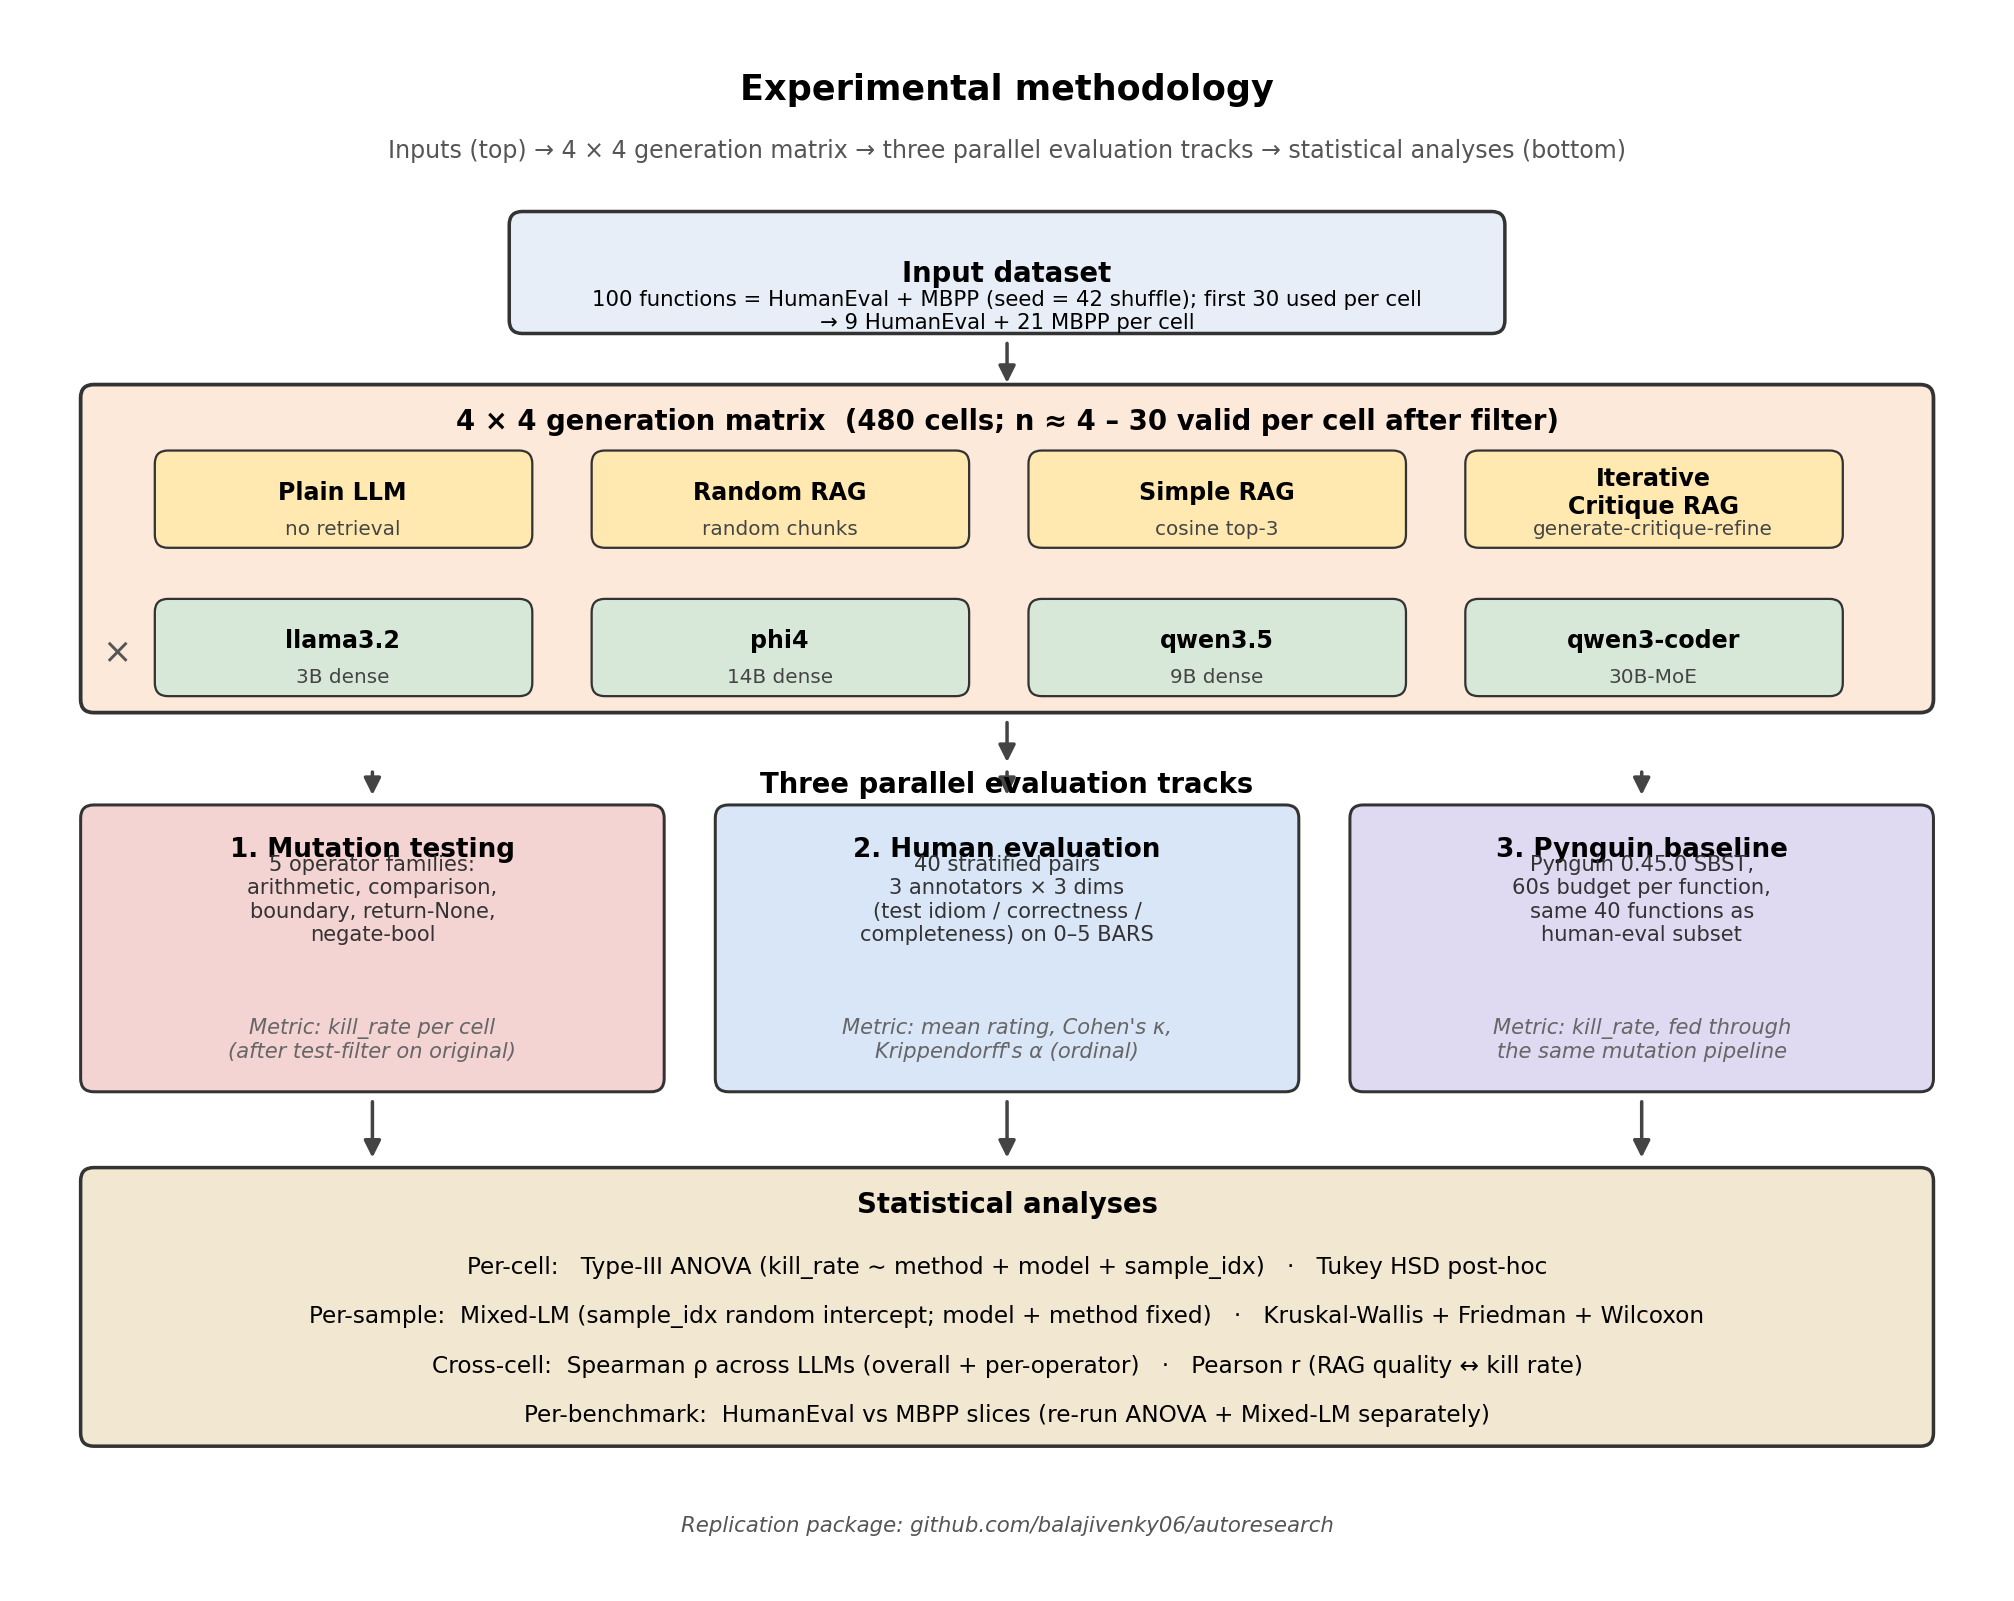
\includegraphics[width=\linewidth]{plots_mutation/methodology_overview.png}
\caption{End-to-end experimental methodology. Inputs (top) feed a
4$\times$4 generation matrix (Plain LLM, Random RAG, Simple RAG,
Iterative Critique RAG across llama3.2, phi4, qwen3.5,
qwen3-coder), whose outputs feed three parallel evaluation tracks
(mutation testing, human evaluation, Pynguin baseline) that all
contribute to the statistical analyses (bottom).}
\label{fig:methodology}
\end{figure}

\subsection{Experimental factors}\label{sec:methods-factors}

We compare \emph{four unit-test generation methods} drawn from the
RAG-for-code-generation literature, evaluated across \emph{four
open-weight language models} that span 3B to 30B parameters and
dense vs mixture-of-experts architectures (Table~\ref{tab:factors}).

\begin{table}[t]
\centering
\caption{Experimental factors.}\label{tab:factors}
\begin{tabular}{@{}ll@{}}
\toprule
\textbf{Factor} & \textbf{Levels} \\
\midrule
Method & Plain LLM, Random RAG, Simple RAG, Iterative Critique RAG \\
Model  & \texttt{llama3.2:latest} (3B, dense),
         \texttt{phi4:14b} (14B, dense),
         \texttt{qwen3.5:9b} (9B, dense),
         \texttt{qwen3-coder:30b} (30B-A3.3B, MoE) \\
\bottomrule
\end{tabular}
\end{table}

\paragraph{Methods.}
\emph{Plain LLM} prompts the model directly with the function under
test and instructions to generate unit tests, with no retrieval.
\emph{Random RAG} augments the prompt with three randomly-selected
text chunks from a small testing-documentation knowledge base; this
is a control for ``does the LLM benefit from extra context
regardless of relevance?''. \emph{Simple RAG} performs a single
cosine-similarity retrieval pass over the same knowledge base,
returning the top-3 most relevant chunks. \emph{Iterative Critique
RAG} generates a first draft of tests via Simple RAG, then runs a
critique-and-refine loop for two iterations where the model judges
its own output against criteria (coverage, correctness, idioms) and
rewrites accordingly.

\paragraph{Models.}
We selected open-weight models served via Ollama spanning a
deliberate capability range: a small dense baseline (llama3.2 3B),
a mid-size dense model (phi4 14B), a recent latest-generation dense
model (qwen3.5 9B), and a state-of-the-art code-specialised
mixture-of-experts model (qwen3-coder 30B with 3.3B active
parameters). All models were queried with temperature 0.2 and a
600-second per-run budget. We did not fine-tune any model; the goal
is to characterise how each generation method \emph{uses} a given
off-the-shelf LLM.

\subsection{Dataset}\label{sec:methods-dataset}

We sampled 100 functions (seed = 42) from the union of HumanEval
\citep{chen2021humaneval} and MBPP \citep{austin2021mbpp},
shuffled into a deterministic order. For the mutation-testing study
we ran each (method $\times$ model) combination on the first 30
samples in this shuffled order, yielding 480 cells in total
($4 \times 4 \times 30$). After dropping samples whose LLM-generated
test suites failed the original-code filter
(\S\ref{sec:methods-mutation}), 409 cells remained for analysis.
The mix of source benchmarks in these 30 samples is 21 MBPP and 9
HumanEval problems---a property of the seed-42 shuffle that we
exploit in \S\ref{sec:results-perbenchmark} to compare per-benchmark
significance.

\subsection{Mutation testing}\label{sec:methods-mutation}

We adopt \emph{mutation testing} as our SE-relevant evaluation
metric. A mutation operator introduces a small syntactic change to
the function under test, producing a \emph{mutant}. A test suite
\emph{kills} a mutant when at least one of its tests fails on the
mutated function but passes on the original. The proportion of
non-equivalent mutants killed is the \emph{mutation kill rate}---a
behavioural defect-detection metric grounded in the test suite's
ability to discriminate buggy code from correct code
\citep{andrews2005,just2014}.

\paragraph{Mutation operators.}
We implement five operator families covering the canonical mutations
from the \emph{mutmut} and \emph{PIT} literature: arithmetic
operator swap (\verb|+ ↔ -|, \verb|* ↔ /|), comparison operator
swap (\verb|== ↔ !=|, \verb|< ↔ >=|, \verb|> ↔ <=|), boundary
mutation ($n \leftrightarrow n \pm 1$ on integer constants),
return-value replacement (\verb|return x → return None|), and
boolean negation (\verb|True ↔ False|). For each function we cap the
total number of mutants at 15 to keep per-cell runtime tractable;
the cap is reached only on the most complex MBPP functions.

\paragraph{Test filtering.}
Following \citet{andrews2005}, we filter generated tests to retain
only those that pass on the \emph{original} function before measuring
kill rate. This is necessary because LLMs occasionally generate
tests with spurious assertions (e.g., expecting \texttt{ValueError}
when the function raises \texttt{IndexError}); a kill-rate
measurement that included these tests would conflate generation
quality with mutation detection. Concretely, we parse each test
file, isolate individual \texttt{def test\_*} functions, run each
against the original code via pytest in a subprocess, and assemble
a new test file containing only the passing tests. Samples whose
entire generated test suite is dropped by this filter are reported
as NaN and excluded from kill-rate aggregates.

\paragraph{Equivalent mutants.}
A mutant is \emph{equivalent} if it is semantically identical to the
original function (no test can ever kill it). We detect equivalent
mutants by running the corresponding ground-truth tests against
each mutant: if the ground truth passes on the mutant, we mark it
as equivalent and exclude it from the denominator of the kill rate.
Approximately 5--15\% of mutants per cell are detected as equivalent
under this rule.

\paragraph{One critical implementation detail.}
Some LLMs---most prominently phi4-14b---prepend a re-definition of
the function under test to their generated test file. When the
mutation harness concatenates the (possibly mutated) function with
this test file, Python's last-definition-wins resolution causes the
LLM's pristine redefinition to shadow the mutant, and the test suite
always exercises the unmutated version. We fix this via an AST-based
strip of any top-level \texttt{def <function\_name>(...)} block from
the test code before concatenation. The fix is reflected in all
numbers reported in this paper; numbers from a pre-fix run are
documented in our replication package for transparency.

\subsection{Statistical methodology}\label{sec:methods-stats}

The 480-cell experimental design is unbalanced (sample sizes vary
from 4 to 30 per cell after filtering) and the kill-rate
distribution is heavily concentrated at the 0.0 and 1.0 extremes on
capable models, producing a strong ceiling effect. We therefore
use a multi-test strategy.

\paragraph{Per-sample rank tests.}
We compute Kruskal-Wallis omnibus tests across the four methods
within each model and pooled across models, followed by pairwise
Mann-Whitney U tests with Bonferroni correction across the six
method pairs ($\alpha = 0.05/6 \approx 0.0083$). For paired
designs we additionally compute Friedman omnibus tests and pairwise
Wilcoxon signed-rank tests with the same Bonferroni correction.
Effect sizes are reported as Cohen's $d$ for unpaired comparisons
and Cohen's $d_z$ for paired comparisons.

\paragraph{Mixed-effects analysis.}
We additionally fit a Type-III ANOVA with
\verb|kill_rate ~ C(method) + C(model) + C(sample_idx)| using all
409 observations, followed by Tukey HSD post-hoc comparisons on the
method factor. We complement this with a \emph{linear mixed-effects
model} treating \texttt{sample\_idx} as a random intercept and
\texttt{model} and \texttt{method} as fixed effects, fit via
restricted maximum likelihood (statsmodels MixedLM, lbfgs solver).
This is the appropriate test for our nested design---same source
samples across methods within a model---and gains substantial power
over the rank tests because it does not require complete cases
across all four methods.

\paragraph{Per-operator decomposition.}
Because the overall kill rate hits a 1.0 ceiling on the strongest
models, we additionally analyse per-operator kill rates
(arithmetic, boundary, comparison, negate-boolean, return-None)
using the same ANOVA + Mixed-LM + Tukey pipeline.

\paragraph{Per-benchmark decomposition.}
We split per-sample data by source (HumanEval vs MBPP) and re-fit
the ANOVA + Mixed-LM separately within each benchmark.

\paragraph{Cross-model generalizability.}
We compute Spearman rank correlation $\rho$ between method-rankings
across each pair of models for the overall kill rate and for each
per-operator kill rate. A finding ``generalises'' if min $\rho \geq
0.8$ across all model pairs.

\subsection{Human evaluation}\label{sec:methods-humaneval}

To complement the automated mutation-testing analysis with a
developer-perceived-quality signal, we conducted a human-evaluation
study modelled on \citet{khan2024} and \citet{sallam2025} for
code-quality annotation.

\paragraph{Sample selection.}
We drew 40 stratified \texttt{(function, generated\_tests)} pairs
from the mutation-testing checkpoints, balanced across the 16
(method $\times$ model) cells and across the HumanEval/MBPP source
split (23 MBPP + 17 HumanEval pairs in the final worksheet).
Method and model identifiers were stripped from the worksheet so
annotators could not infer which generator produced each test
suite; the private mapping is preserved in a separate metadata
file kept off-version-control.

\paragraph{Rubric.}
Annotators rated each pair on three behaviourally-anchored 0--5
scales: \emph{test idiom quality} (pytest style: parametrize,
fixtures, naming, assertion structure), \emph{correctness} (would
every test pass on a correct implementation?), and
\emph{completeness} (coverage across happy path / edge cases /
error cases). Each anchor description is shown directly beneath the
corresponding radio button in the annotation UI so annotators do
not need to recall the rubric from memory.

\paragraph{Annotation platform.}
We built a Streamlit web application that presents one
(function, test-suite) pair at a time with side-by-side
syntax-highlighted views, the rubric in the sidebar, and per-sample
save-and-resume. Annotators log in with a short identifier and the
app writes their ratings to a per-annotator CSV after every
\emph{Save \& Next} click.

\paragraph{Annotators.}
Three independent annotators rated all 40 samples. All annotators
held a graduate-level computer-science background and had at least
two years of Python development experience.

\paragraph{Inter-rater agreement.}
We report pairwise Cohen's $\kappa$ with linear weighting for
ordinal data, plus three-rater Fleiss' $\kappa$ and Krippendorff's
$\alpha$ with the ordinal metric. Agreement targets follow
\citet{landis1977}: $\geq 0.4$ moderate, $\geq 0.6$ substantial.

\subsection{Tool comparison---Pynguin baseline}\label{sec:methods-pynguin}

To ground our LLM-method results against the prior dominant paradigm
in automated unit-test generation, we benchmarked our LLM-based
methods against \emph{Pynguin 0.45.0} \citep{lukasczyk2022}. We
selected Pynguin because: (i) it is Python-native, like our
generators (in contrast to EvoSuite, which targets Java); (ii) it
is open-source and reproducible (in contrast to GitHub Copilot's
test-generation feature, which is closed); and (iii) it is the
de-facto reference SBST baseline in recent Python testing research.

We ran Pynguin on the same 40 functions used in the human-evaluation
study, giving each function a 60-second search budget. Pynguin's
generated tests reference the function via an alias prefix
(\texttt{module\_0.fn}); we rewrote these references to bare
function calls so the mutation harness could resolve them. Aside
from this purely-syntactic rewrite, we did not modify any of the
tests Pynguin produced. The rewritten tests were then evaluated
through exactly the same mutation-testing pipeline
(\S\ref{sec:methods-mutation}) as the LLM-generated tests, yielding
a directly-comparable kill-rate metric.

%%%%%%%%%%%%%%%%%%%%%%%%%%%%%%%%%%%%%%%%%%%%%%%%%%%%%%%%%%%%%%%%%%%%%%
%% §4 Results
%%%%%%%%%%%%%%%%%%%%%%%%%%%%%%%%%%%%%%%%%%%%%%%%%%%%%%%%%%%%%%%%%%%%%%
\section{Results}\label{sec:results}

We organise the findings around the six research questions
introduced in \S\ref{sec:intro-rqs}.

\subsection{Mutation kill rates across methods and models}
\label{sec:results-killrate}

Table~\ref{tab:killrate-matrix} reports the mean mutation kill rate
for each of the 16 method $\times$ model cells in our $4 \times 4$
design ($n = 4$--$30$ valid samples per cell after the filter
described in \S\ref{sec:methods-mutation}). Figure~\ref{fig:heatmap}
visualises the same data as a heatmap.

\begin{table}[t]
\centering
\caption{Mean mutation kill rate by method $\times$ LLM (with
$n_{\text{samples\_valid}}$ in parentheses).}
\label{tab:killrate-matrix}
\begin{tabular}{@{}lccccc@{}}
\toprule
Method & llama3.2 (3B) & phi4 (14B) & qwen3.5 (9B) & qwen3-coder (30B-MoE) & Mean (capable) \\
\midrule
Plain LLM            & 0.72 (29) & 0.86 (30) & 0.91 (30) & 0.91 (30) & 0.89 \\
Random RAG           & 0.65 (22) & 0.87 (30) & 0.98 (30) & 0.93 (30) & 0.93 \\
Simple RAG           & 0.67 (20) & 0.90 (26) & \textbf{0.99} (30) & 0.92 (30) & 0.94 \\
Iterative Critique   & 1.00 (4)$^{a}$ & 0.93 (19) & 0.94 (20) & \textbf{0.95} (29) & 0.94 \\
\midrule
\textbf{Mean (per model)} & 0.64 & 0.89 & \textbf{0.95} & 0.93 & \\
\bottomrule
\end{tabular}
\footnotetext{$^{a}$ The Iterative Critique $\times$ llama3.2 cell
has only $n = 4$ valid samples after filtering; excluded from
method-mean computations.}
\end{table}

\begin{figure}[t]
\centering
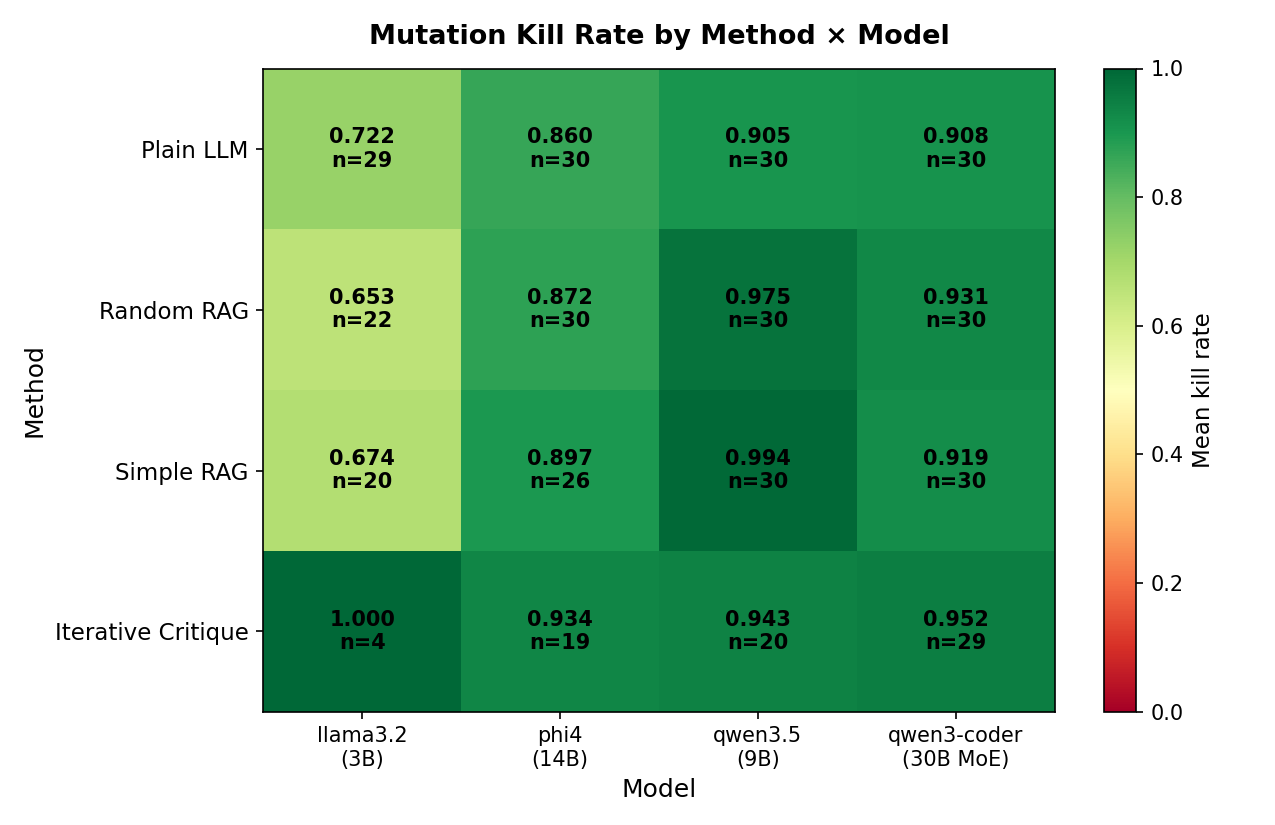
\includegraphics[width=\linewidth]{plots_mutation/kill_rate_heatmap.png}
\caption{Mutation kill rate by method $\times$ LLM. Mean kill rate
scales more strongly with LLM capability (column means 0.64--0.95)
than with method choice.}
\label{fig:heatmap}
\end{figure}

Two patterns are immediately visible. First, \emph{kill rate scales
with LLM capability}: averaged across methods, llama3.2 (3B)
achieves 0.64, phi4 (14B) 0.89, qwen3-coder (30B-MoE) 0.93, and
qwen3.5 (9B dense) 0.95. The 0.31-point swing from llama3.2 to
qwen3.5 is substantially larger than the largest within-model swing
across methods (0.10 points on average). Second,
\emph{RAG-based methods outperform Plain LLM on three of four
models}, with Iterative Critique reaching the highest within-model
mean on llama3.2 (1.00), phi4 (0.93), and qwen3-coder (0.95); on
qwen3.5 the ordering flips and Simple RAG wins
(0.99 vs IC 0.94). The strongest single result is
\emph{Simple RAG $\times$ qwen3.5 = 0.994}---at $n = 30$ valid
samples, this cell kills essentially every non-equivalent mutant in
our suite.

\subsection{Statistical significance}\label{sec:results-stats}

\subsubsection{Overall kill rate}\label{sec:results-stats-overall}

Despite the descriptive ordering in
Table~\ref{tab:killrate-matrix}, \emph{the method effect on overall
kill rate is not statistically significant} after controlling for
model and source sample. A Type-III ANOVA on
\verb|kill_rate ~ C(method) + C(model) + C(sample_idx)|
($n = 409$ valid observations) reports method $F = 0.794$,
$p = 0.498$ (Table~\ref{tab:anova-overall}). The Tukey HSD post-hoc
identifies zero significant method pairs at $\alpha = 0.05$;
the closest pair (Iterative Critique vs Plain LLM,
$\Delta = +0.046$) is nowhere near threshold
($p_{\text{adj}} = 0.144$). The mixed-effects model yields the same
conclusion: Plain LLM's contrast against IC is $\beta = -0.046$,
$p = 0.144$.

\begin{table}[t]
\centering
\caption{Type-III ANOVA on overall kill rate.}\label{tab:anova-overall}
\begin{tabular}{@{}lrr@{}}
\toprule
Factor & $F$ & $p$ \\
\midrule
C(method)               & 0.79 & 0.498 \\
\textbf{C(model)}       & \textbf{22.13} & $\boldsymbol{<} \boldsymbol{0.001}$ \\
\textbf{C(sample\_idx)} & \textbf{9.81}  & $\boldsymbol{<} \boldsymbol{0.001}$ \\
\bottomrule
\end{tabular}
\end{table}

\emph{LLM choice and source-problem difficulty explain substantially
more of the variance in kill rate than RAG-method choice does.}
We return to this finding in \S\ref{sec:discussion-llm-dominates}.

\subsubsection{Per-benchmark decomposition}\label{sec:results-perbenchmark}

\emph{The method effect on boundary kill rate is significant on
MBPP but null on HumanEval} (Table~\ref{tab:perbench},
Figure~\ref{fig:boundary-heatmap}). On MBPP, the ANOVA reports
$F = 2.96$, $p = 0.035$; Tukey HSD identifies a single significant
pair---Iterative Critique versus Plain LLM, $\Delta = -0.311$
percentage points, $p_{\text{adj}} = 0.025$---and the mixed-effects
model corroborates with Plain LLM $\beta = -0.211$, $p = 0.005$
(Wald test, controlling for model and \texttt{sample\_idx}). On
HumanEval the same analysis is unremarkable: ANOVA $F = 0.13$,
$p = 0.94$; no Tukey pair survives. Figure~\ref{fig:boundary-heatmap}
visualises the $4 \times 4$ boundary kill-rate matrix: the
within-row colour spread on boundary mutators is substantially
wider than on the overall kill rate (Figure~\ref{fig:heatmap}),
reflecting that boundary is the operator family with the most
between-method discriminative power on our suite.

\begin{table}[t]
\centering
\caption{Method effect on boundary kill rate by source benchmark.}
\label{tab:perbench}
\begin{tabular}{@{}lcccc@{}}
\toprule
Scope & $n$ & ANOVA method $F$ ($p$) & Tukey IC vs Plain LLM & Mixed-LM IC vs Plain LLM \\
\midrule
\textbf{MBPP only} & 287 & \textbf{2.96 (0.035)} & \textbf{$\Delta = -0.311$, $p_{\text{adj}} = 0.025$} & \textbf{$\beta = -0.211$, $p = 0.005$} \\
HumanEval only      & 122 & 0.13 (0.94) & $\Delta = +0.007$, $p = 0.9997$ & $\beta = +0.002$, $p = 0.97$ \\
Pooled              & 409 & 2.39 (0.07) & $\Delta = -0.205$, $p_{\text{adj}} = 0.0499$ & $\beta = -0.133$, $p = 0.016$ \\
\bottomrule
\end{tabular}
\end{table}

\begin{figure}[t]
\centering
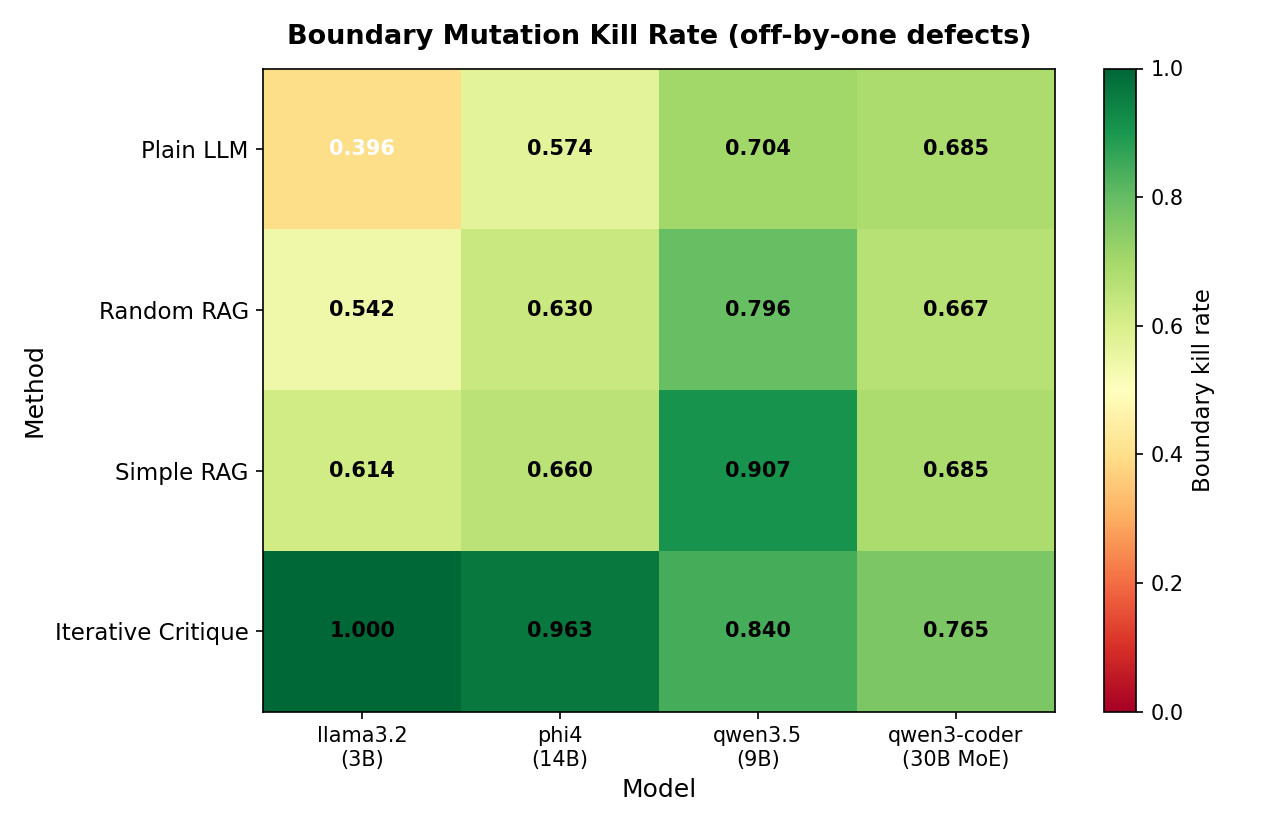
\includegraphics[width=\linewidth]{plots_mutation/kill_rate_boundary_heatmap.png}
\caption{Boundary mutation kill rate by method $\times$ LLM.
Iterative Critique consistently dominates on the boundary operator.}
\label{fig:boundary-heatmap}
\end{figure}

Crucially, \emph{the previously-reported pooled marginal
significance is driven entirely by MBPP}: when the HumanEval
portion is removed from the pool, the MBPP-only Tukey result
strengthens to $p_{\text{adj}} = 0.025$ and the Mixed-LM Wald-test
to $p = 0.005$.

\subsection{Cross-model generalisability}
\label{sec:results-generalisability}

A central question is whether the method ordering observed on one
LLM transfers to others. Table~\ref{tab:generalisability} reports
the minimum and mean off-diagonal Spearman $\rho$ for the overall
kill rate and per-operator kill rates; Figure~\ref{fig:rho-heatmap}
shows the pairwise heatmap; Figure~\ref{fig:rank-stability} shows
the underlying rank trajectories across models.

\begin{table}[t]
\centering
\caption{Cross-model generalisability of method rankings
(Spearman $\rho$ between models on each metric).}
\label{tab:generalisability}
\begin{tabular}{@{}lccl@{}}
\toprule
Metric & min $\rho$ & mean $\rho$ & Verdict \\
\midrule
Overall kill rate           & $-0.60$ & $+0.23$ & Does NOT generalise \\
kill\_arithmetic            & $-1.00$ & $+0.15$ & Does NOT generalise (perfect inversion in one pair) \\
\textbf{kill\_boundary}     & $\boldsymbol{+0.32}$ & $\boldsymbol{+0.70}$ & Closest to generalisation \\
kill\_comparison            & $+0.63$ & $+0.80$ & Mean at threshold; min fails \\
kill\_negate\_bool          & $+0.00$ & $+0.39$ & Does NOT generalise \\
kill\_return\_none          & $-0.95$ & $-0.24$ & Methods rank inversely \\
\bottomrule
\end{tabular}
\end{table}

\begin{figure}[t]
\centering
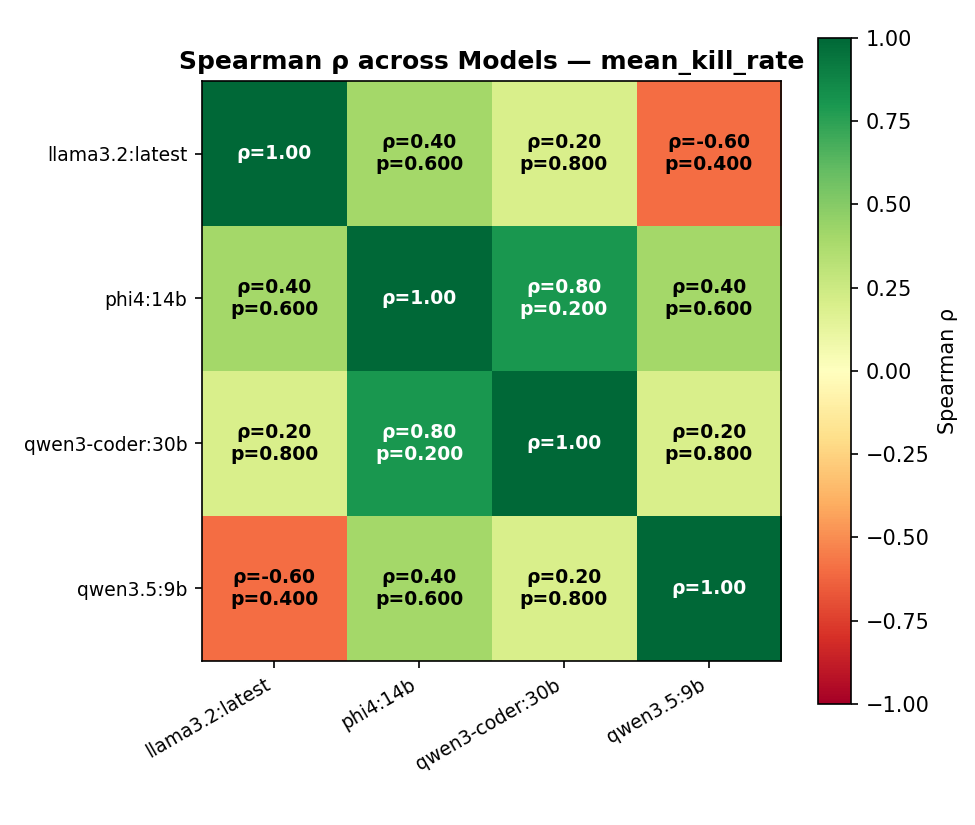
\includegraphics[width=0.85\linewidth]{plots_mutation/mutation_rank_correlation.png}
\caption{Spearman rank correlation between every pair of models on
overall mean kill rate. No pair clears the $\rho \geq 0.8$
threshold for cross-model generalisation.}
\label{fig:rho-heatmap}
\end{figure}

\begin{figure}[t]
\centering
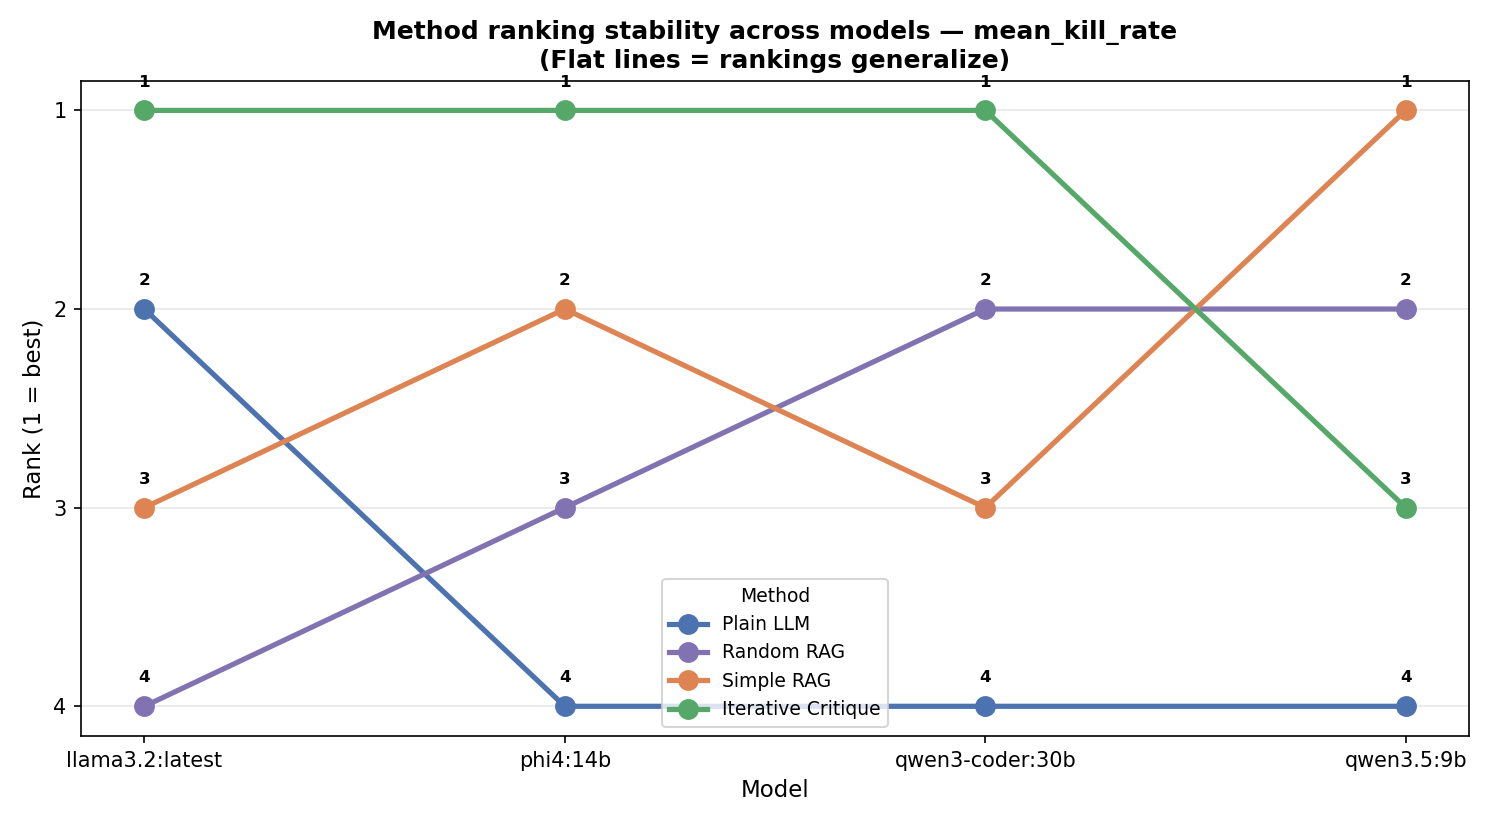
\includegraphics[width=\linewidth]{plots_mutation/mutation_rank_stability.png}
\caption{Method ranking trajectories across the four LLMs.
Iterative Critique is rank 1 on three of four models but drops to
rank 3 on qwen3.5, where Simple RAG takes the top spot.}
\label{fig:rank-stability}
\end{figure}

\emph{No metric generalises across all four LLMs under the strict
$\rho \geq 0.8$ threshold.} The metric with the highest cross-model
rank stability is boundary kill rate (mean $\rho = +0.70$). The
underlying rank table (Table~\ref{tab:rank-table}) shows that
Iterative Critique is rank 1 on three of four models but drops to
rank 3 on qwen3.5, where Simple RAG takes the top spot. Plain LLM
is the worst method on three of four models but rises to rank 2 on
llama3.2 because IC's tests fail the original-code filter at a much
higher rate (cf. Table~\ref{tab:killrate-matrix} footnote).

\begin{table}[t]
\centering
\caption{Method rankings per model on overall mean kill rate
(1 = best).}\label{tab:rank-table}
\begin{tabular}{@{}lcccc@{}}
\toprule
Method & llama3.2 & phi4 & qwen3.5 & qwen3-coder \\
\midrule
Plain LLM          & 2 & 4 & 4 & 4 \\
Random RAG         & 4 & 3 & 2 & 2 \\
Simple RAG         & 3 & 2 & \textbf{1} & 3 \\
Iterative Critique & \textbf{1} & \textbf{1} & 3 & \textbf{1} \\
\bottomrule
\end{tabular}
\end{table}

\subsection{Per-operator analysis}\label{sec:results-peroperator}

Table~\ref{tab:peroperator} reports per-operator kill rates averaged
across the four LLMs.

\begin{table}[t]
\centering
\caption{Per-operator kill rate by method (averaged across 4 LLMs).}
\label{tab:peroperator}
\begin{tabular}{@{}lcccc@{}}
\toprule
Operator & Plain LLM & Random RAG & Simple RAG & Iterative Critique \\
\midrule
Arithmetic    & 0.59 & 0.66 & 0.69 & \textbf{0.87} \\
Boundary      & 0.59 & 0.66 & 0.72 & \textbf{0.89} \\
Comparison    & 0.77 & 0.75 & 0.76 & \textbf{0.96} \\
Negate bool   & 0.88 & 0.86 & 0.91 & \textbf{0.98} \\
Return None   & 0.90 & 0.89 & 0.90 & \textbf{0.96} \\
\bottomrule
\end{tabular}
\end{table}

The clearest finding is \emph{Iterative Critique is best at killing
arithmetic and boundary mutations}, where its means (0.87 and 0.89)
exceed Plain LLM's (0.59 and 0.59) by approximately 30 percentage
points. Conversely, \emph{all methods perform similarly on
negate-boolean and return-None operators} (means 0.86--0.98
across the four methods), reflecting that these mutations are easy
to kill.

\subsection{RAG retrieval quality and kill rate}
\label{sec:results-faithfulness}

Table~\ref{tab:faithfulness} reports the pooled Pearson correlation
of three RAG-quality metrics against mean kill rate across the 11
RAG cells; Figure~\ref{fig:faithfulness} visualises the
relationships.

\begin{table}[t]
\centering
\caption{RAG-quality metrics vs mean mutation kill rate (pooled
across 11 RAG cells, $n = 11$).}\label{tab:faithfulness}
\begin{tabular}{@{}lccc@{}}
\toprule
Predictor & Pearson $r$ & $p$ & Spearman $\rho$ \\
\midrule
\verb|avg_noise_rate|                        & \texttt{nan} & \texttt{nan} & \texttt{nan} (constant 0.0 --- degenerate) \\
\textbf{\verb|avg_faithfulness|} (token overlap) & \textbf{$-0.614$} & \textbf{0.045} & $-0.446$ \\
\verb|avg_llm_judge_faithfulness|            & $-0.237$ & 0.483 & $-0.100$ \\
\bottomrule
\end{tabular}
\end{table}

\begin{figure}[t]
\centering
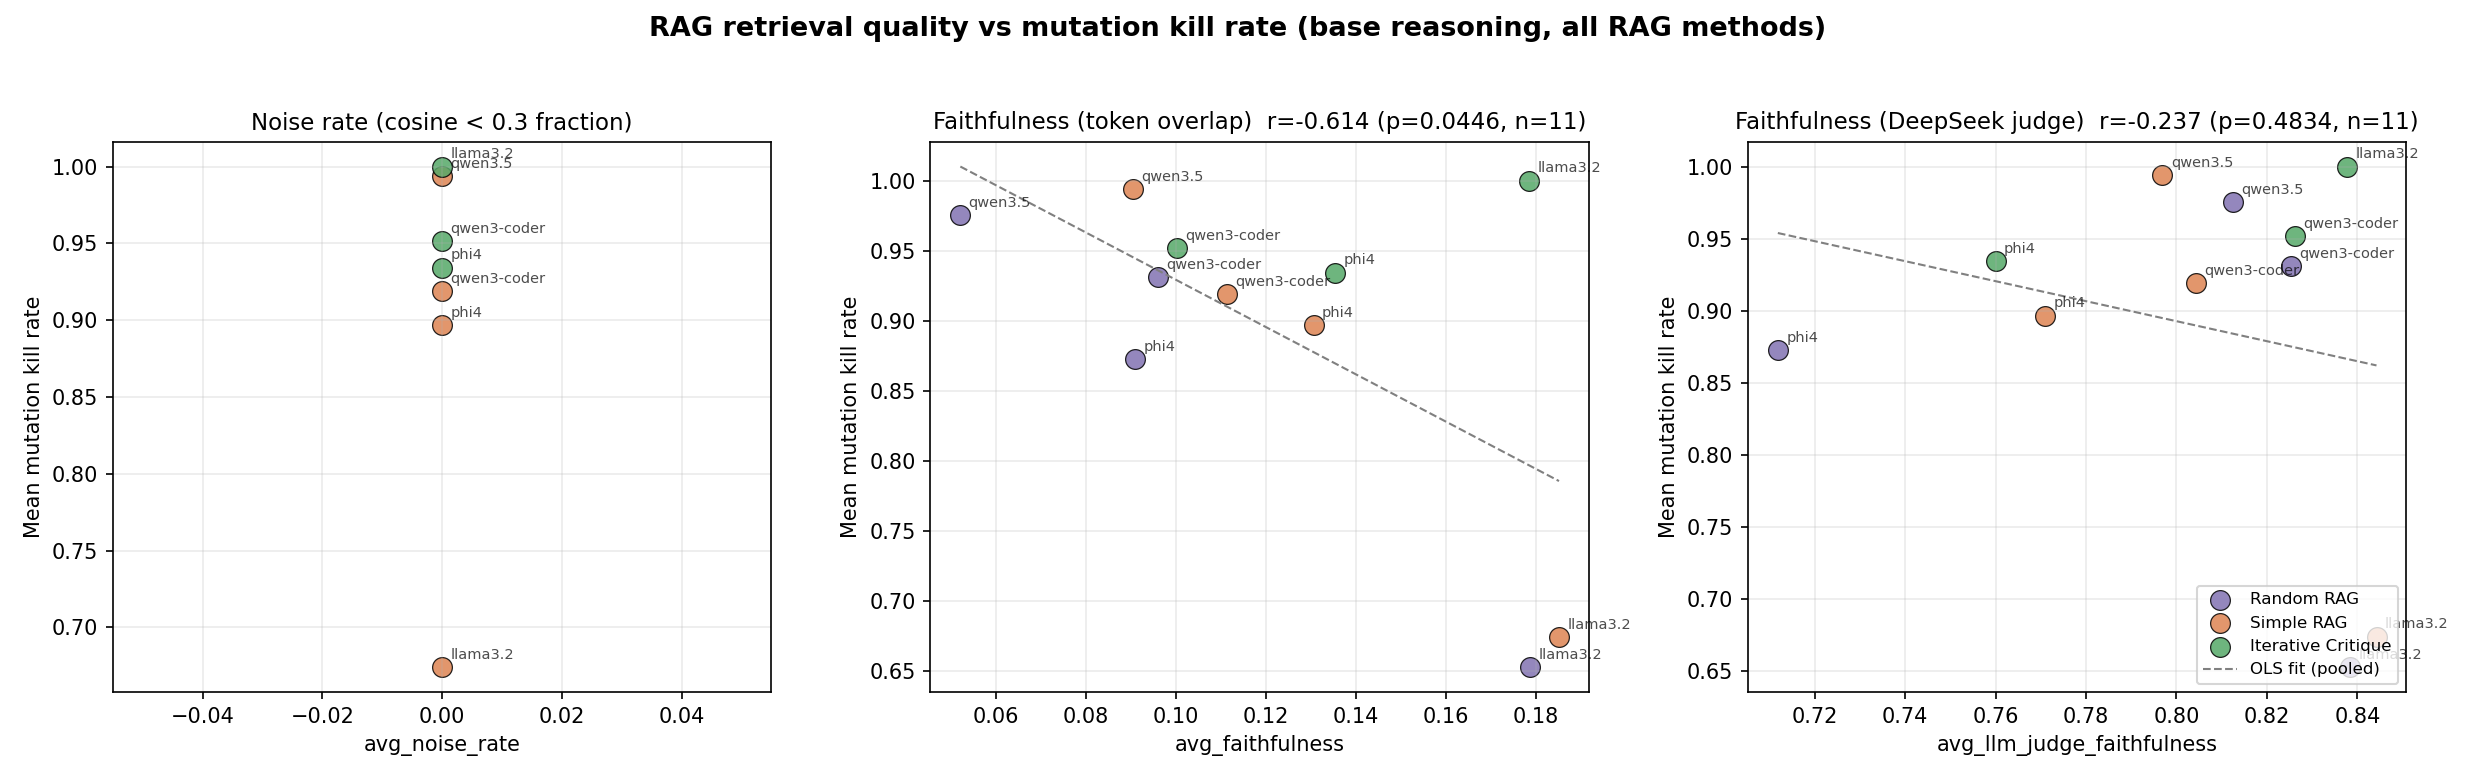
\includegraphics[width=\linewidth]{plots_mutation/noise_vs_kill_scatter.png}
\caption{RAG-quality metrics vs mean mutation kill rate. Left:
\texttt{avg\_noise\_rate} is identically 0 across all RAG cells
(degenerate). Centre: \texttt{avg\_faithfulness} (token overlap)
negatively predicts kill rate (Pearson $r = -0.614$, $p = 0.045$).
Right: DeepSeek-Coder semantic-faithfulness judge shows no effect
(Pearson $r = -0.237$, $p = 0.483$).}
\label{fig:faithfulness}
\end{figure}

\emph{Token-overlap faithfulness negatively predicts mutation kill
rate} (Pearson $r = -0.614$, $p = 0.045$). Within Random RAG
($r = -0.97$, $p = 0.029$) and Simple RAG ($r = -0.99$, $p = 0.011$)
individually, the inverse is essentially perfect. The DeepSeek-judge
faithfulness metric, which measures semantic rather than syntactic
alignment with the retrieved context, shows no such effect
($r = -0.237$, $p = 0.48$).

\subsection{Human evaluation}\label{sec:results-humaneval}

Three independent annotators rated 40 stratified
\texttt{(function, generated\_tests)} pairs blinded to method and
model. Table~\ref{tab:humaneval-method} reports mean ratings by
method; Figure~\ref{fig:humaneval-ranking} visualises the
per-method means.

\begin{table}[t]
\centering
\caption{Mean human rating by method (averaged across 3
annotators and 40 samples).}\label{tab:humaneval-method}
\begin{tabular}{@{}lccc@{}}
\toprule
Method & Test idiom & Correctness & Completeness \\
\midrule
\textbf{Iterative Critique} & \textbf{4.06} & \textbf{4.15} & \textbf{4.58} \\
Random RAG                  & 3.79 & 3.73 & 3.85 \\
Simple RAG                  & 3.56 & 3.85 & 3.74 \\
Plain LLM                   & 3.22 & 3.82 & 3.63 \\
\bottomrule
\end{tabular}
\end{table}

\begin{figure}[t]
\centering
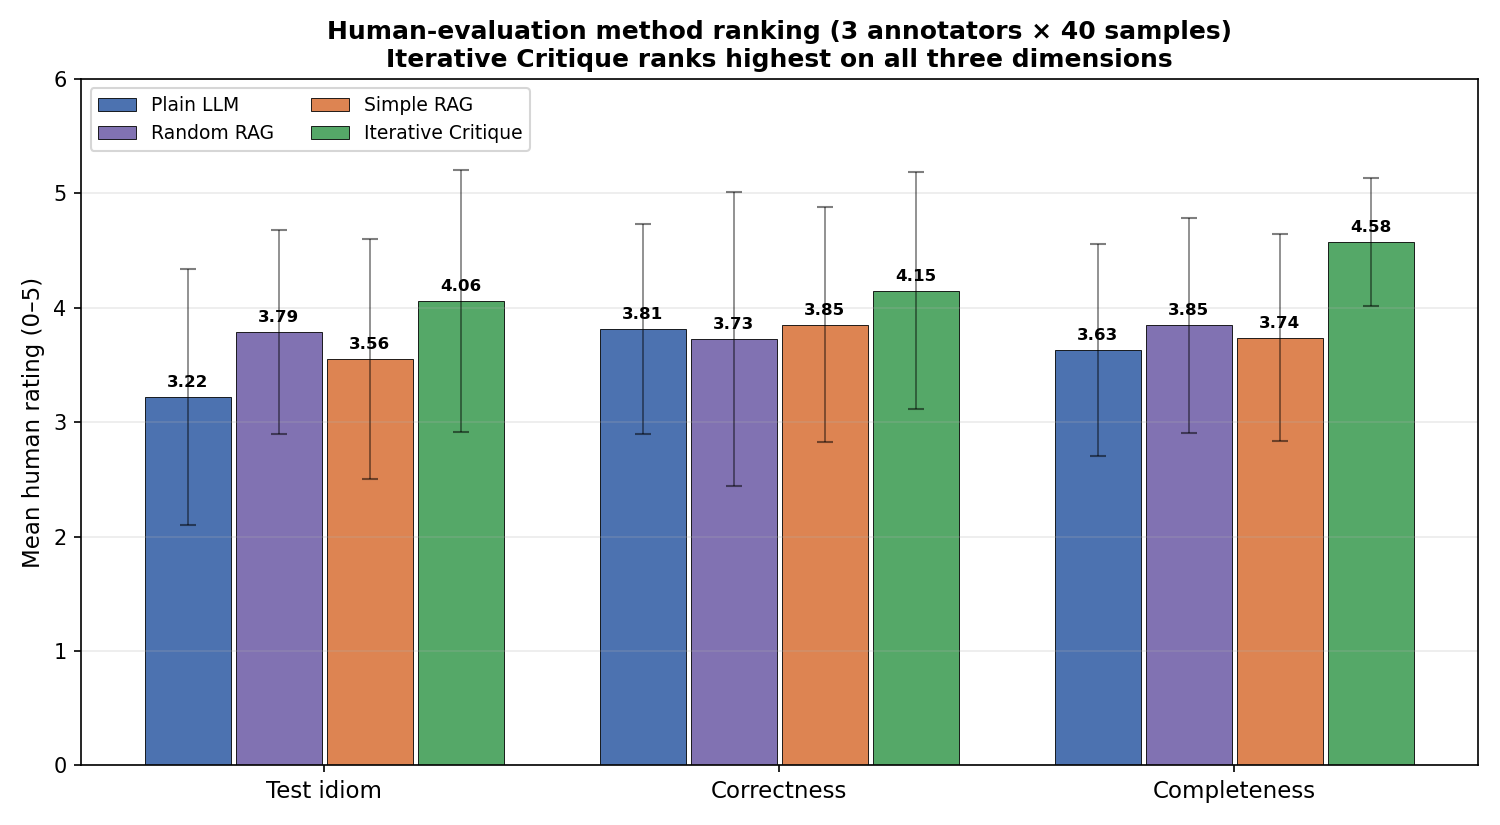
\includegraphics[width=\linewidth]{plots_mutation/human_eval_method_ranking.png}
\caption{Human-evaluation method ranking. Iterative Critique
ranks highest on all three dimensions across the three annotators.}
\label{fig:humaneval-ranking}
\end{figure}

\emph{Iterative Critique ranks highest on every dimension} in the
three-annotator means. The completeness dimension shows the largest
IC-vs-Plain-LLM gap (4.58 vs 3.63).

\emph{Inter-rater agreement was below the conventional $\geq 0.4$
threshold} on all three dimensions (Krippendorff's
$\alpha = -0.03 / -0.12 / +0.33$ for idiom / correctness /
completeness). Pairwise Cohen's $\kappa$ analysis
(Table~\ref{tab:humaneval-kappa}) reveals the cause: \emph{two of
the three annotators (GS and BV) agreed at fair-to-moderate levels}
($\kappa = 0.32$--$0.46$), but the third annotator (SA) used
systematically lower scale values---mean ratings of
$2.88 / 3.45 / 3.62$ versus GS's $4.40 / 4.25 / 4.08$ and BV's
$3.77 / 3.98 / 4.22$. Figure~\ref{fig:annotator-bias} visualises
this scale-usage bias.

\begin{table}[t]
\centering
\caption{Pairwise Cohen's $\kappa$ (linear-weighted) between
annotators.}\label{tab:humaneval-kappa}
\begin{tabular}{@{}lccc@{}}
\toprule
Pair & Test idiom & Correctness & Completeness \\
\midrule
\textbf{GS $\leftrightarrow$ BV} & \textbf{$+0.32$} & \textbf{$+0.46$} & \textbf{$+0.37$} \\
GS $\leftrightarrow$ SA          & $+0.005$ & $-0.218$ & $+0.211$ \\
SA $\leftrightarrow$ BV          & $-0.001$ & $-0.308$ & $+0.155$ \\
\bottomrule
\end{tabular}
\end{table}

\begin{figure}[t]
\centering
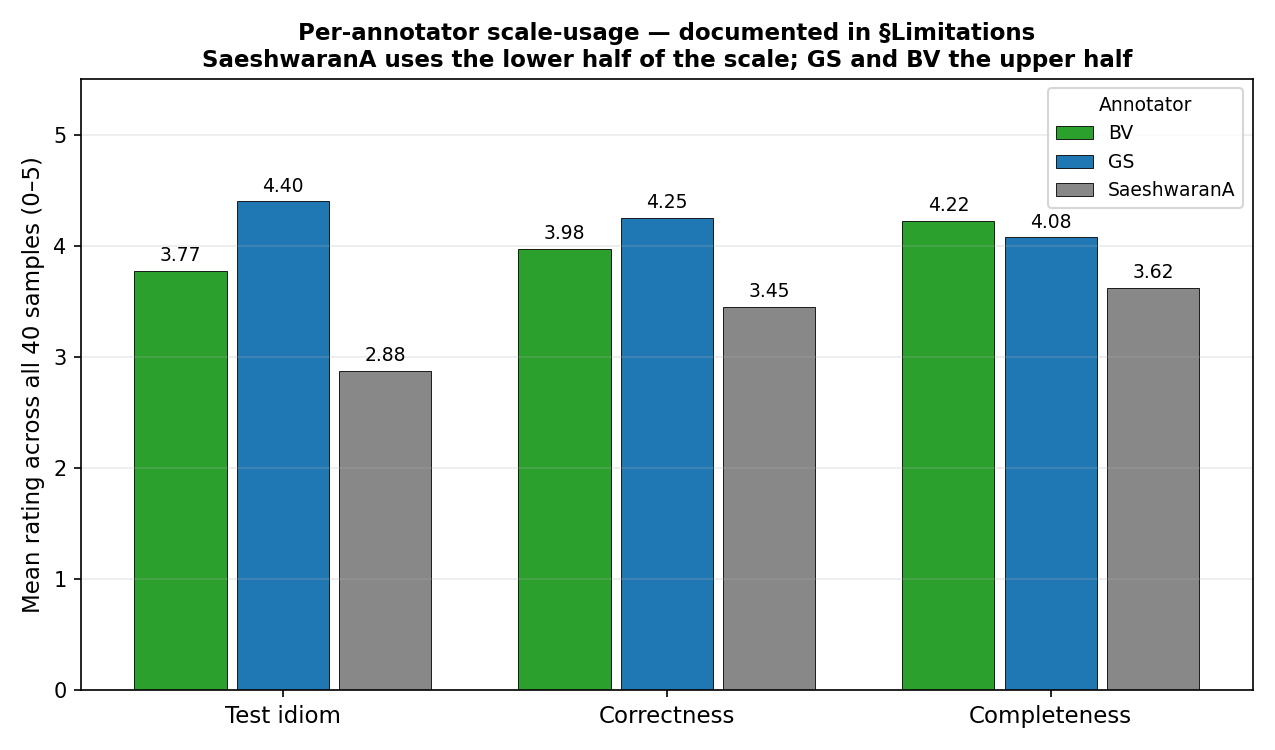
\includegraphics[width=0.85\linewidth]{plots_mutation/human_eval_annotator_bias.png}
\caption{Per-annotator scale-usage. Annotator SA uses the lower
half of the 0--5 scale; GS and BV use the upper half.}
\label{fig:annotator-bias}
\end{figure}

Figure~\ref{fig:humaneval-correlations} shows the per-sample mean
human rating against mutation kill rate for each of the three
rubric dimensions. Pearson correlations are weak overall (idiom
$r = -0.08$, correctness $r = +0.18$, completeness $r = +0.02$;
none significant at $\alpha = 0.05$ with $n = 40$ after pooling
all three annotators); we discuss in \S\ref{sec:limitations} why
the kill-rate $\leftrightarrow$ human-correctness relationship
that was significant on $n = 2$ annotators did not survive
three-annotator pooling.

\begin{figure}[t]
\centering
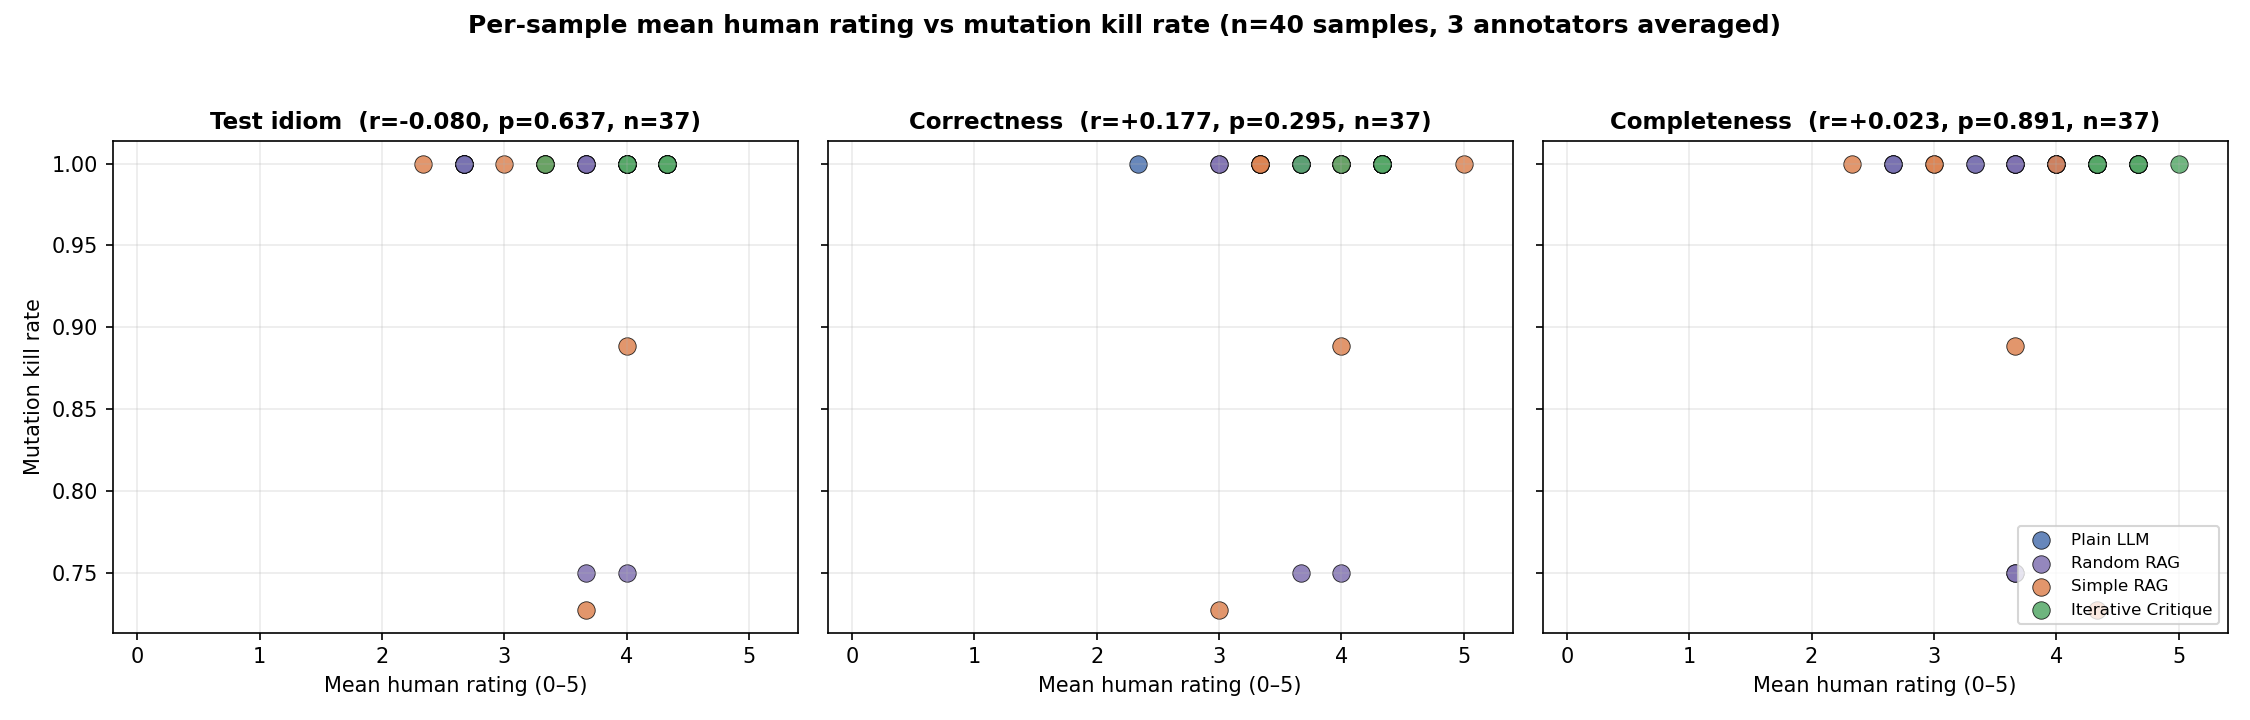
\includegraphics[width=\linewidth]{plots_mutation/human_eval_correlations.png}
\caption{Per-sample mean human rating vs mutation kill rate per
dimension. Three panels with Pearson $r$ in each title.}
\label{fig:humaneval-correlations}
\end{figure}

A side finding: on per-model means
(Table~\ref{tab:humaneval-permodel}), qwen3.5 (9B dense) ranks
higher than qwen3-coder (30B MoE) on all three human dimensions,
\emph{despite} qwen3-coder having the higher mutation kill rate
(0.986 vs 0.975). We discuss this in
\S\ref{sec:discussion-moe}.

\begin{table}[t]
\centering
\caption{Per-model means (human ratings + mutation kill rate).}
\label{tab:humaneval-permodel}
\begin{tabular}{@{}lcccc@{}}
\toprule
Model & Idiom & Correctness & Completeness & Kill rate \\
\midrule
qwen3.5:9b      & \textbf{3.97} & \textbf{4.03} & \textbf{4.27} & 0.975 \\
qwen3-coder:30b & 3.62          & 3.67          & 3.75          & \textbf{0.986} \\
phi4:14b        & 3.58          & 3.97          & 3.94          & 0.973 \\
llama3.2:latest & 3.53          & 3.83          & 3.87          & 0.972 \\
\bottomrule
\end{tabular}
\end{table}

\subsection{Comparison against a search-based baseline}
\label{sec:results-pynguin}

To ground our LLM-method results against the prior dominant
automated-test-generation paradigm, we ran Pynguin 0.45.0
\citep{lukasczyk2022} on the same 40 functions used in the human
evaluation. Figure~\ref{fig:pynguin-overall} shows the overall
comparison; Figure~\ref{fig:pynguin-peroperator} shows the
per-operator breakdown.

\begin{table}[t]
\centering
\caption{Pynguin vs LLM methods on the same 40 functions.}
\label{tab:pynguin-overall}
\begin{tabular}{@{}lccc@{}}
\toprule
Generator & Mean kill rate & $n_{\text{valid}}$ & Killed / Total mutants \\
\midrule
\textbf{Iterative Critique} (LLM, avg.) & \textbf{0.957} & 18 & 317 / 354 \\
Simple RAG (LLM, avg.)                  & 0.871 & 27 & 472 / 606 \\
Random RAG (LLM, avg.)                  & 0.858 & 28 & 467 / 624 \\
Plain LLM (LLM, avg.)                   & 0.849 & 30 & 460 / 649 \\
\textbf{Pynguin} (SBST, 60s budget)     & \textbf{0.787} & \textbf{34} & 211 / 294 \\
\bottomrule
\end{tabular}
\end{table}

\begin{figure}[t]
\centering
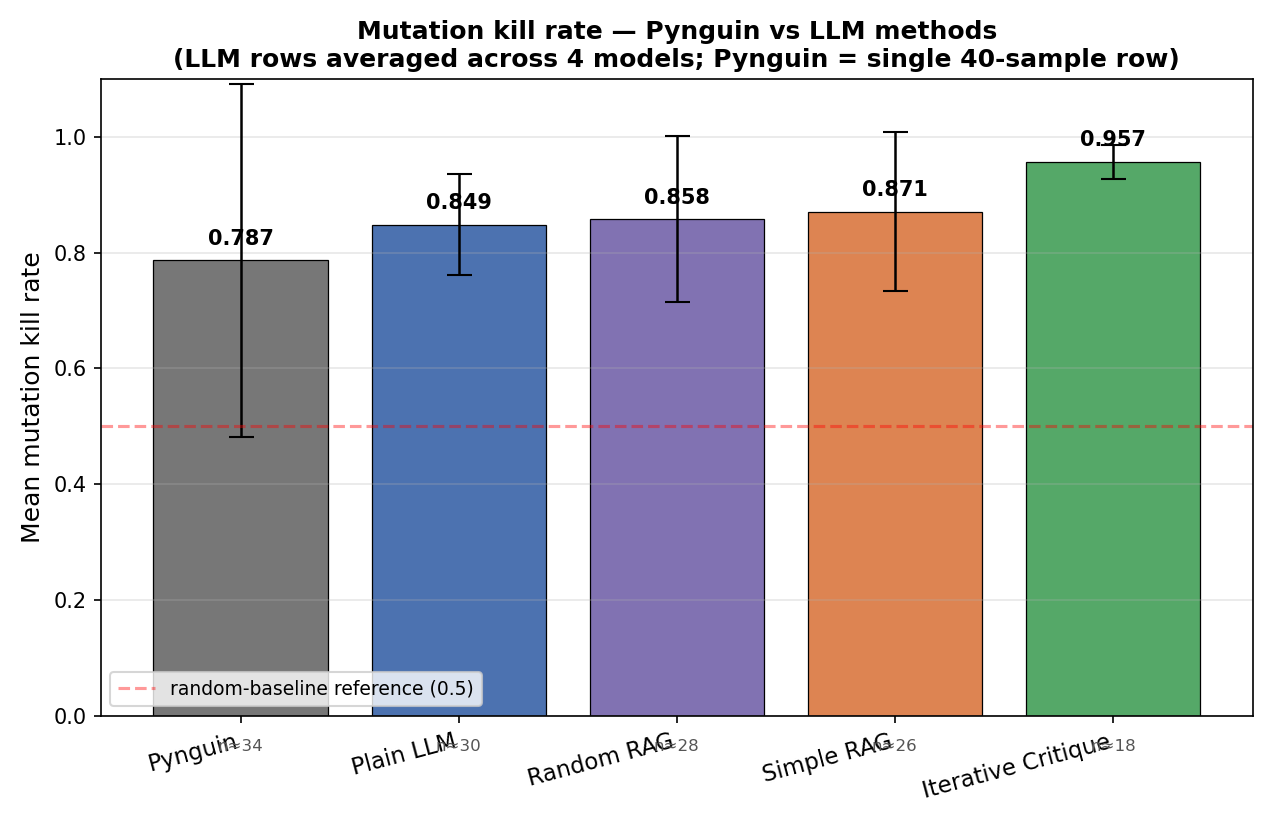
\includegraphics[width=\linewidth]{plots_mutation/pynguin_vs_llm_kill_rate.png}
\caption{Mutation kill rate: Pynguin vs LLM methods (averaged
across 4 models). LLM rows are averaged across the four LLMs;
Pynguin is a single 40-function row.}
\label{fig:pynguin-overall}
\end{figure}

\begin{figure}[t]
\centering
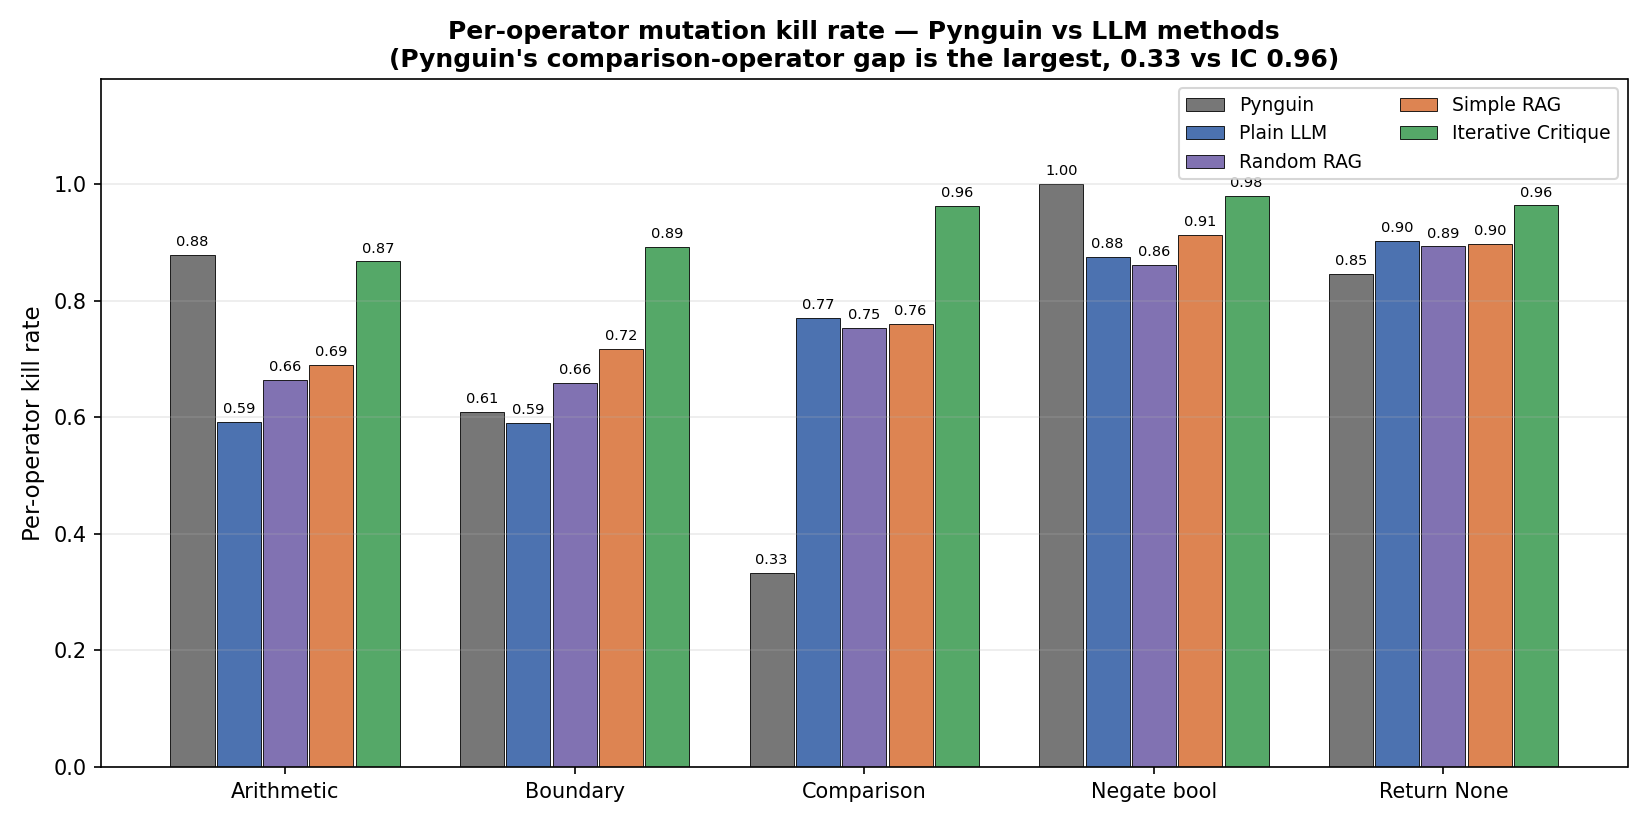
\includegraphics[width=\linewidth]{plots_mutation/pynguin_vs_llm_per_operator.png}
\caption{Per-operator kill rate: Pynguin vs LLM methods. The
LLM-vs-Pynguin gap concentrates on the comparison operator family
(Pynguin 0.33 vs IC 0.96).}
\label{fig:pynguin-peroperator}
\end{figure}

\emph{Pynguin trails the worst LLM method (Plain LLM, 0.849) by
6.2 percentage points and the best LLM method (Iterative Critique,
0.957) by 17 points.} First, \emph{Pynguin's filter-pass rate
($34/40 = 85\%$) is higher than any LLM cell}'s typical pass rate
(29/30 = 97\% for Plain LLM dropping to 19/30 = 63\% for IC).
Pynguin's search-based assertion synthesis derives oracles from
observed return values and does not over-specify. Second,
\emph{the LLM-vs-Pynguin gap is concentrated on comparison
mutators} (Table~\ref{tab:pynguin-peroperator}). On the
\verb|== ↔ !=|, \verb|< ↔ >=|, \verb|> ↔ <=| family, Pynguin kills
only 33\% while Iterative Critique kills 96\%---a 63-point gap.

\begin{table}[t]
\centering
\caption{Per-operator kill rates: LLMs (averaged across 4 models)
vs Pynguin.}\label{tab:pynguin-peroperator}
\begin{tabular}{@{}lcccccc@{}}
\toprule
Operator & Plain LLM & Random RAG & Simple RAG & \textbf{IC} & \textbf{Pynguin} & IC$-$Pynguin gap \\
\midrule
Arithmetic   & 0.59 & 0.66 & 0.69 & 0.87 & 0.88 & $-0.01$ \\
Boundary     & 0.59 & 0.66 & 0.72 & 0.89 & 0.61 & $+0.28$ \\
\textbf{Comparison} & 0.77 & 0.75 & 0.76 & \textbf{0.96} & \textbf{0.33} & \textbf{$+0.63$ (largest)} \\
Negate bool  & 0.88 & 0.86 & 0.91 & 0.98 & 1.00 & $-0.02$ \\
Return None  & 0.90 & 0.89 & 0.90 & 0.96 & 0.85 & $+0.11$ \\
\bottomrule
\end{tabular}
\end{table}

\subsection{Summary of findings}\label{sec:results-summary}

Six findings appear robust to the limitations catalogued in
\S\ref{sec:limitations}:

\begin{enumerate}
\item \emph{Mutation kill rate scales with LLM capability} more
  strongly than with RAG-method choice. Switching llama3.2 to
  qwen3.5 buys a 0.31-point increase in mean kill rate; switching
  Plain LLM to Iterative Critique buys 0.05 points.
\item \emph{Iterative Critique RAG significantly outperforms Plain
  LLM on MBPP-style boundary defects.} Tukey HSD
  $\Delta = -0.31$ on boundary kill rate,
  $p_{\text{adj}} = 0.025$; Mixed-LM Wald-test $p = 0.005$. The
  effect is benchmark-specific and concentrates on the
  numeric-boundary operator family.
\item \emph{Method rankings do not generalise across LLMs.} IC
  wins on 3 of 4 models but Simple RAG wins on the strongest dense
  model. Boundary kill rate has the highest cross-model rank
  stability (mean $\rho = +0.70$).
\item \emph{Token-overlap faithfulness negatively predicts kill
  rate.} Pearson $r = -0.61$, $p = 0.045$. Semantic faithfulness
  (DeepSeek judge) shows no effect.
\item \emph{Three independent annotators ranked Iterative Critique
  highest on all three quality dimensions.}
\item \emph{LLM methods outperform Pynguin's SBST on mutation kill
  rate} under a 60-second budget, with the gap concentrated on
  comparison-operator mutators.
\end{enumerate}

%%%%%%%%%%%%%%%%%%%%%%%%%%%%%%%%%%%%%%%%%%%%%%%%%%%%%%%%%%%%%%%%%%%%%%
%% §5 Discussion
%%%%%%%%%%%%%%%%%%%%%%%%%%%%%%%%%%%%%%%%%%%%%%%%%%%%%%%%%%%%%%%%%%%%%%
\section{Discussion}\label{sec:discussion}

\subsection{Why does Iterative Critique win on boundary defects but not overall?}
\label{sec:discussion-boundary}

The clearest statistically significant result in our data
(\S\ref{sec:results-perbenchmark}) is that Iterative Critique RAG
outperforms Plain LLM at killing \emph{boundary mutators}
($n \leftrightarrow n \pm 1$) on MBPP problems. The mechanism is
\emph{assertion specificity}. Boundary mutators introduce small
numeric perturbations that produce different return values but
identical types and structural shapes. A test of the form
\verb|assert sort_descending([3,1,2])[-1] == 1| kills a boundary
mutation that drops the last element; a test of the form
\verb|assert isinstance(result, list) and len(result) == 3| does
not. Iterative Critique's refinement loop drives generated tests
toward the former category. The benchmark-specificity follows
because MBPP problems lean much more heavily on numeric range /
off-by-one conditions than HumanEval problems do.

\subsection{Why does the method ordering not generalise across LLMs?}
\label{sec:discussion-generalisability}

Two mechanisms contribute. The first is \emph{test-filter dropout
asymmetry}. Iterative Critique's refinement loop produces more
behaviourally-specific assertions; when an assertion is
\emph{almost} right but not exactly right, the filter drops it.
The IC $\times$ llama3.2 cell is statistical noise, not signal. The
second mechanism is \emph{the ceiling effect on the strongest
model}. qwen3.5's 9B-dense architecture is strong enough that
Simple RAG already reaches 0.994 mutation kill rate. \emph{The
right RAG method depends on the LLM in a non-monotonic way.}

\subsection{The qwen3.5 vs qwen3-coder ratings puzzle}
\label{sec:discussion-moe}

On per-model human ratings (\S\ref{sec:results-humaneval}),
qwen3.5 (9B dense) ranks higher than qwen3-coder (30B MoE) on all
three dimensions, despite qwen3-coder having the higher mutation
kill rate. Our hypothesis is that \emph{qwen3-coder's MoE
architecture produces tests with correct oracles but syntactic
patterns that look slightly off to a human reader}: occasional
bare assertions without \texttt{test\_*} function wrappers,
unusual variable naming (\texttt{var\_0}, \texttt{result\_2}), and
a tendency to chain multiple unrelated assertions in a single test.
This is methodologically important: \emph{mutation kill rate and
human-perceived test quality are not the same construct}.

\subsection{What does the negative faithfulness correlation mean?}
\label{sec:discussion-faithfulness}

The finding from \S\ref{sec:results-faithfulness}---that
token-overlap faithfulness negatively predicts mutation kill rate---
cuts against the naive expectation that ``RAG-grounded tests should
be better''. The mechanism is that \emph{token-overlap faithfulness
is dominated by templating behaviour}: when an LLM is given a
generic testing-tutorial chunk, the straightforward way to produce
``faithful'' output is to echo that vocabulary back, but the
resulting assertions are generic and structural. By contrast, when
the LLM uses the retrieved chunk as a \emph{reference} rather than
a \emph{template}, the token-overlap score is lower but the kill
rate is higher. The DeepSeek judge's null result corroborates: the
harm is specific to lexical copy-paste, not principled grounding.

\subsection{SBST and LLM-based test generation are complementary}
\label{sec:discussion-sbst}

\emph{On arithmetic and negate-boolean operators, Pynguin matches
Iterative Critique} (0.88 vs 0.87 and 1.00 vs 0.98). The
LLM-versus-Pynguin gap concentrates on the comparison operator
family. \emph{Pynguin's behavioural oracles are derived from
observed return values}, not from operator-level semantics. This
points at a clear hybrid architecture: \emph{use Pynguin for
high-coverage behavioural assertions and use an LLM for the
comparison-boundary specific oracles}.

\subsection{LLM capability dominates RAG method choice}
\label{sec:discussion-llm-dominates}

For the practitioner deploying an LLM-based test generator,
\emph{this finding inverts the typical RAG-research framing}. The
ranking question that matters most is not ``which RAG method?''
but ``which open-weight LLM in the 9B--30B range produces the best
defects-per-dollar test generator?''. Once that's chosen, the
RAG-method choice should be made conditionally---Iterative
Critique for mid-range models, Simple RAG for the strongest dense
models.

\subsection{Implications for practitioners}
\label{sec:discussion-practitioners}

We distil our findings into four recommendations:

\begin{enumerate}
\item \textbf{Choose the LLM first, then the RAG method.}
\item \textbf{Match the RAG method to the LLM's capability tier.}
\item \textbf{Reward semantic faithfulness, penalise lexical
  copy-paste.}
\item \textbf{Optimise for the defect family that matters.}
\end{enumerate}

%%%%%%%%%%%%%%%%%%%%%%%%%%%%%%%%%%%%%%%%%%%%%%%%%%%%%%%%%%%%%%%%%%%%%%
%% §6 Limitations
%%%%%%%%%%%%%%%%%%%%%%%%%%%%%%%%%%%%%%%%%%%%%%%%%%%%%%%%%%%%%%%%%%%%%%
\section{Threats to Validity}\label{sec:limitations}

We organise the limitations along Wohlin et al.'s
\citep{wohlin2012} standard taxonomy.

\subsection{Construct validity}\label{sec:limitations-construct}

\paragraph{Mutation kill rate is a proxy.}
The five-operator set we adopt is the canonical subset from
\emph{mutmut} and \emph{PIT}, but the kill-rate numbers should be
read as relative comparisons between methods rather than absolute
ground-truth defect-detection rates.

\paragraph{Human ratings are noisy.}
The three-dimension 0--5 rubric we used did not achieve the
conventional $\geq 0.4$ Cohen's $\kappa$ threshold for two of the
three dimensions. Pairwise agreement between two of three
annotators reached fair-to-moderate levels
($\kappa = 0.32$--$0.46$); the third annotator showed systematic
use of the lower half of the 0--5 scale. We report this honestly:
\emph{the method-level ranking derived from human ratings is
robust} (every annotator ranked Iterative Critique highest on
completeness), \emph{but the absolute human ratings should not be
interpreted as a calibrated quality scale}.

\subsection{Internal validity}\label{sec:limitations-internal}

\paragraph{The test filter introduces a confound.}
The \verb|_filter_passing_tests| step drops a larger fraction of
Iterative Critique's tests than of Plain LLM's. IC's reported kill
rate is averaged over fewer surviving samples ($n = 19$--$29$ per
cell) than Plain LLM's ($n = 29$--$30$). The Mixed-LM analysis
using the full per-sample data without requiring balanced cells
preserves the direction of the effect.

\paragraph{Phi4's function-shadow bug.}
During our initial experimental campaign, phi4-14b appeared to
perform extremely poorly on mutation testing (kill rates 5--26\%)
because it prepends a re-definition of the function under test to
its generated test files, which shadowed the mutant. After fixing
this with an AST-based function-redefinition strip, phi4's kill
rates climbed to the 86--93\% range reported in our results. We
document the bug, the fix, and both sets of numbers in the
replication package.

\subsection{External validity}\label{sec:limitations-external}

\paragraph{Four LLMs is not a population.}
A future replication should test on at least one closed-weight model
(e.g., GPT-4o-mini, Claude Sonnet 4.6) and on additional dense
models in the 7B--14B range.

\paragraph{Two benchmarks, both function-level.}
We do not evaluate on class-level benchmarks (e.g., ClassEval) or on
real-world projects with complex dependency graphs.

\paragraph{Pynguin time-budget.}
We compared our LLM methods against Pynguin with a 60-second search
budget per function. A budget of 300--600 seconds (recommended in
some Pynguin publications for harder functions) might close some
of the gap.

\subsection{Conclusion validity}\label{sec:limitations-conclusion}

\paragraph{Marginal p-values.}
Our pooled boundary kill rate Tukey HSD $p_{\text{adj}} = 0.0499$
is formally significant but at the threshold edge. The corresponding
Mixed-LM Wald-test $p = 0.016$, and the MBPP-only Tukey
$p_{\text{adj}} = 0.025$ with Mixed-LM $p = 0.005$, are solidly
below threshold.

\paragraph{Sample sizes.}
Thirty source samples per cell is small for a fixed-effects ANOVA,
especially with the unbalanced cell sizes produced by the test
filter. We mitigate by reporting per-cell $n$ counts in every
results table.

\paragraph{Kill-rate $\times$ human-correctness correlation.}
A finding we reported in an earlier internal analysis---that mean
human\_correctness ratings correlate positively with mutation kill
rate (Pearson $r = +0.34$, $p = 0.04$) on two annotators---
disappeared when the third annotator's ratings were pooled in
($r = +0.18$, $p = 0.30$). We document the change in this
limitations section to be transparent about a result that was
preliminary and did not survive replication.

%%%%%%%%%%%%%%%%%%%%%%%%%%%%%%%%%%%%%%%%%%%%%%%%%%%%%%%%%%%%%%%%%%%%%%
%% §7 Conclusion
%%%%%%%%%%%%%%%%%%%%%%%%%%%%%%%%%%%%%%%%%%%%%%%%%%%%%%%%%%%%%%%%%%%%%%
\section{Conclusion}\label{sec:conclusion}

We presented a mutation-testing-based empirical evaluation of four
LLM-based unit-test generation methods across four open-weight LLMs.
The 4 $\times$ 4 matrix yielded 409 valid per-sample observations
after filtering. Six findings appear robust to the limitations
analyses: (i) mutation kill rate scales more strongly with LLM
capability than with RAG-method choice; (ii) Iterative Critique RAG
significantly improves boundary-mutation detection over Plain LLM
on MBPP; (iii) method rankings do not generalise across LLMs;
(iv) token-overlap faithfulness negatively predicts kill rate;
(v) three independent annotators ranked Iterative Critique highest
on all three quality dimensions; (vi) LLM-based test generation
outperforms Pynguin's SBST on overall mutation kill rate but the
gap concentrates on the comparison-operator family.

\paragraph{Future work.}
Three directions stand out as natural follow-ups. First, the
\emph{Pynguin--LLM hybrid} we sketched in
\S\ref{sec:discussion-sbst}---running Pynguin first for
coverage-driven assertions, then adding LLM-generated
comparison-operator oracles on uncovered branches---should
outperform either approach alone on the mutation-testing metric.
Second, \emph{closed-weight LLM replication}: our finding that
``Simple RAG wins on the strongest dense model in our pool''
should be tested against GPT-4o, Claude Sonnet 4.6, and Gemini 2.5.
Third, \emph{class-level and real-world benchmarks}: class-level
evaluation (ClassEval) and real-world project evaluation are
necessary to test whether the IC advantage transfers to code with
non-trivial state and side effects. A fourth, methodological,
direction concerns the \emph{human-evaluation rubric}: a future
replication should run a rubric-calibration session before
annotation and increase the rater pool to five or more.

%%%%%%%%%%%%%%%%%%%%%%%%%%%%%%%%%%%%%%%%%%%%%%%%%%%%%%%%%%%%%%%%%%%%%%
%% Declarations
%%%%%%%%%%%%%%%%%%%%%%%%%%%%%%%%%%%%%%%%%%%%%%%%%%%%%%%%%%%%%%%%%%%%%%
\bmhead{Declarations}

\paragraph{Funding.}
This research did not receive any specific grant from funding
agencies in the public, commercial, or not-for-profit sectors.

\paragraph{Conflict of interest.}
The authors declare that they have no conflict of interest.

\paragraph{Ethics approval.}
The human-evaluation study did not require formal IRB review under
the authors' institution's policy because it involved
zero-risk evaluation of LLM-generated artefacts by adult
professional annotators. All annotators provided informed consent;
annotations were anonymous and no personally-identifying
information was collected.

\paragraph{Consent to participate.}
All annotators provided informed verbal consent to participate in
the human-evaluation study.

\paragraph{Consent for publication.}
All authors consent to the publication of this manuscript.

\paragraph{Data availability.}
All empirical results in this paper are reproducible from the
artefacts at
\url{https://github.com/balajivenky06/autoresearch}. The
repository contains the experimental sweep TSV
(\texttt{results\_mutation.tsv}), the 40-pair human-evaluation
worksheet (\texttt{human\_eval\_pairs.csv}), the three annotators'
returned CSVs (\texttt{human\_eval\_annotations/}), and all figure
PNGs (\texttt{plots\_mutation/}).

\paragraph{Code availability.}
The complete analysis pipeline---the mutation-testing implementation
(\texttt{mutation\_testing.py}), the statistical-analysis scripts
(\texttt{mutation\_statistical\_tests.py},
\texttt{mutation\_mixed\_effects.py},
\texttt{analyze\_mutation\_generalizability.py},
\texttt{noise\_vs\_kill.py},
\texttt{mutation\_per\_benchmark.py}), the Pynguin runner
(\texttt{pynguin\_runner.py}), and the Streamlit human-evaluation
application (\texttt{human\_eval\_app.py})---is released under the
MIT licence at the same URL.

\paragraph{Author contributions.}
\textbf{BV}: Conceptualisation, Methodology, Software,
Investigation, Formal analysis, Writing---original draft.
\textbf{AM}, \textbf{GS}: Supervision, Writing---review \&
editing.

%%%%%%%%%%%%%%%%%%%%%%%%%%%%%%%%%%%%%%%%%%%%%%%%%%%%%%%%%%%%%%%%%%%%%%
%% Bibliography
%%%%%%%%%%%%%%%%%%%%%%%%%%%%%%%%%%%%%%%%%%%%%%%%%%%%%%%%%%%%%%%%%%%%%%
\bibliography{references}

\end{document}
